% manuscript.tex -- Canadian Journal of Fisheries and Aquatic Sciences, Research article
% Compile with: latexmk -pdf manuscript.tex   (biblatex + biber)
% Every number in the text, tables and captions is listed with its source in number_check.md.
\documentclass[12pt,letterpaper,fleqn]{article}
\usepackage[T1]{fontenc}
\usepackage[utf8]{inputenc}
\usepackage{lmodern}
\usepackage[margin=1in]{geometry}
\usepackage{setspace}
\usepackage{lineno}
\usepackage{amsmath}
\setlength{\mathindent}{0pt}
\usepackage{graphicx}
\usepackage{booktabs}
\usepackage{tabularx}
\usepackage{array}
\usepackage{etoolbox}
\usepackage{adjustbox}
\usepackage[labelfont=bf,labelsep=period,font=small,justification=raggedright,singlelinecheck=false]{caption}
\usepackage[english]{babel}
\usepackage{csquotes}
\usepackage[style=authoryear,backend=biber,maxcitenames=2,mincitenames=1,maxbibnames=99,
  giveninits=true,uniquename=false,uniquelist=false,dashed=false,doi=true,url=true,
  isbn=false,eprint=false,sorting=nyt,date=year,useprefix=true]{biblatex}
\usepackage[hidelinks]{hyperref}
% --- approximation of the CJFAS (Harvard, author-year) reference style -------------------
% In text: (Bundy and Fanning 2005), (Frank et al. 2011). In the list:
% Bundy, A., and Fanning, L.P. 2005. Title. Journal, 62(7): 1474--1489. doi:10.1139/f05-086.
\DeclareNameAlias{sortname}{family-given}
\DeclareNameAlias{default}{family-given}
\renewrobustcmd*{\bibinitdelim}{}
\DeclareDelimFormat{nameyeardelim}{\addspace}
\DeclareDelimFormat[bib,biblist]{finalnamedelim}{\addcomma\addspace\bibstring{and}\space}
\DeclareDelimFormat[bib,biblist]{multinamedelim}{\addcomma\space}
\renewbibmacro*{date+extradate}{%
  \iffieldundef{labelyear}{}{\printtext{\printlabeldateextra}}}
\DeclareFieldFormat*{title}{#1\isdot}
\DeclareFieldFormat{journaltitle}{#1}
\DeclareFieldFormat[article]{volume}{#1}
\DeclareFieldFormat[article]{number}{\mkbibparens{#1}}
\DeclareFieldFormat{pages}{#1}
\renewcommand*{\bibpagespunct}{\addcolon\space}
\renewbibmacro*{in:}{}
\renewbibmacro*{volume+number+eid}{%
  \printfield{volume}\printfield{number}\setunit{\addcomma\space}\printfield{eid}}
\renewbibmacro*{journal+issuetitle}{%
  \usebibmacro{journal}\setunit*{\addcomma\space}%
  \iffieldundef{series}{}{\newunit\printfield{series}\setunit{\addspace}}%
  \usebibmacro{volume+number+eid}\setunit{\addspace}\usebibmacro{issue+date}%
  \setunit{\addcolon\space}\usebibmacro{issue}\newunit}
\DeclareFieldFormat{doi}{doi\addcolon\href{https://doi.org/#1}{\nolinkurl{#1}}}
\DeclareFieldFormat{url}{\url{#1}}
\DeclareFieldFormat{urldate}{}
\AtEveryBibitem{\clearfield{month}\clearfield{issn}\clearlist{language}\clearfield{urlyear}}
% internal bookkeeping notes in references.bib are not printed
\DeclareSourcemap{\maps[datatype=bibtex]{
  \map{\step[fieldsource=note, match=\regexp{^(Closest|A\sversion|R\spackage|Report\sof|Read\sas|Scanned|English\sedition|Published\sMarch)}, final]
       \step[fieldset=note, null]}}}
\DeclareSortingNamekeyTemplate{\keypart{\namepart{prefix}}\keypart{\namepart{family}}\keypart{\namepart[inits]{given}}}
\setcounter{biburllcpenalty}{7000}
\setcounter{biburlucpenalty}{8000}
\setcounter{biburlnumpenalty}{8000}
\addbibresource{references.bib}

% layout: double-spaced text, continuous line numbers, page numbers
\doublespacing
\linenumbers
\AtBeginEnvironment{table}{\singlespacing\small}
\AtBeginEnvironment{tabularx}{\renewcommand{\arraystretch}{1.15}}
\newcolumntype{L}{>{\raggedright\arraybackslash}X}
\newcolumntype{R}{>{\raggedleft\arraybackslash}X}
\setlength{\parindent}{1.5em}

\newcommand{\yr}{yr$^{-1}$}
\makeatletter\g@addto@macro\UrlBreaks{\do\_}\makeatother
\newcommand{\gm}{g\,m$^{-2}$}

\begin{document}
\sloppy

% ---------------------------------------------------------------------------
\begin{titlepage}
\begin{flushleft}
\textbf{Article type:} Research article\\[1.5em]
{\Large\bfseries A weak, conditional trap: a size-spectrum test of predator--prey role reversal as the cause of non-recovery of Atlantic Cod on the eastern Scotian Shelf\par}
\vspace{2em}
% ------------------------------------------------------------------------------------------
% PLACEHOLDER AUTHOR BLOCK -- to be completed by the author(s). No names or affiliations
% have been invented. Replace every item in square brackets.
% ------------------------------------------------------------------------------------------
\textbf{[AUTHOR NAME(S) -- PLACEHOLDER]}$^{1}$\\[0.8em]
$^{1}$[Affiliation, address, country -- PLACEHOLDER]\\[1.5em]
\textbf{Corresponding author:} [Name, postal address, e-mail address -- PLACEHOLDER]\\[1.5em]
\textbf{Running head:} Role reversal and eastern Scotian Shelf cod\\[1.5em]
\textbf{ORCID:} [PLACEHOLDER]\\[1.5em]
\textbf{Word counts:} abstract 169; main text (Introduction to Discussion) about 7300; reference list about 1900. Four tables, seven figures; supplementary material in a separate file.
\end{flushleft}
\end{titlepage}

% ---------------------------------------------------------------------------
\section*{Abstract}
Atlantic Cod (\textit{Gadus morhua}) on the eastern Scotian Shelf did not recover after the 1993 moratorium, while forage fish increased. One proposed explanation is predator--prey role reversal: released forage fish eat or outcompete young cod. We tested it with a seven-species size-spectrum model calibrated to 1980--85 survey biomasses, cod landings and Scotian Shelf plankton data. Purely size-based predation gave forage fish a negligible role in cod early life, so we added an untested vulnerability factor making forage fish cause 5.9\% of cod deaths between 1~mg and 1~g. Under documented fishing the model did not reproduce non-recovery: cod regained half its 1980--85 spawning biomass two years after the closure, and forage fish rose 1.4-fold against 7.9-fold observed. A weak cod-free alternative stable state existed, but no hindcast reached it. Elevated adult natural mortality reproduced the decline. Forage fishing restored cod only from the alternative state; from the modelled collapsed state it delayed recovery by 2--4 years. In this model, role reversal traps cod only under narrow, unobserved conditions.

\paragraph{Key words:} Atlantic Cod, forage fish, cultivation--depensation, alternative stable states, size-spectrum model, mizer, natural mortality

% ---------------------------------------------------------------------------
\section{Introduction}

Atlantic Cod (\textit{Gadus morhua}, hereafter cod) on the eastern Scotian Shelf (NAFO Subdivision 4Vs and Division 4W, hereafter 4VsW) supported landings of 50--57~kt per year in 1981--86 \autocite{fanning2003assessment}. Survey-based spawning stock biomass (SSB) peaked at 172~kt in 1984 and fell to 4.7~kt by 2002, a 97\% decline \autocite{fanning2003assessment}. The directed fishery closed on 1 September 1993 \autocite{mohn1994assessment}, and fishing mortality on ages 5--15 has since averaged about 0.035~\yr{} and fallen to about 0.01 \autocite{mohn2012laurentian}. Yet the stock did not rebuild. A strong 2004 year class and a fall in natural mortality lifted SSB to 64~kt in 2009 \autocite{swain2012forage,mohn2012laurentian}, but SSB has been below the 50~kt limit reference point in every other year since 1992 \autocite{dfo2011rpa}. The summer survey index was 8.2~kt in 2023 and 4.7~kt in 2024 \autocite{dfo2025rvtrends}. The Laurentian South population of Atlantic Cod, which includes 4VsW cod, was assessed as Endangered in 2010 \autocite{cosewic2010cod}. Slow recovery after collapse is common in gadids \autocite{hutchings2000collapse}, but here the ecosystem also changed around the cod.

As cod and other large demersal fish declined, the shelf shifted towards small pelagic fish and macroinvertebrates \autocite{choi2004transition,frank2005trophic}. The ratio of pelagic to demersal feeders in mass-balance models rose from 0.3 in 1980--85 to 3.0 in 1995--2000 \autocite{bundy2005structure}. The forage-fish complex rose to about ten times its pre-collapse biomass and then declined after it outstripped its zooplankton food \autocite{frank2011transient}. Capelin (\textit{Mallotus villosus}) reappeared on the shelf from the late 1980s during cold anomalies \autocite{frank1996recent}, and the mean individual size and condition of demersal fish fell \autocite{zwanenburg2000effects,choi2004transition}.

Several explanations have been proposed for the failed recovery. The first is predator--prey role reversal, or cultivation--depensation. Abundant adult predators crop the forage fish that eat or compete with their young, and when the adults are fished down the released forage fish depress the survival of the next predator generations \autocite{walters2001cultivation}. For eastern Scotian Shelf cod, \textcite{bundy2005can} described a ``vicious circle'' in which small cod compete with abundant forage fish for a declining prey base and may be eaten by them. Negative relationships between pelagic biomass and cod recruitment have been reported in the southern Gulf of St Lawrence \autocite{swain2000pelagic} and across several North Atlantic regions \autocite{minto2012interactions}, and North Sea herring has been proposed to hold cod in a herring-dominated state \autocite{fauchald2010predator}. The second explanation is elevated adult natural mortality. Natural mortality of 4VsW cod aged 5 and older averaged about 0.8~\yr{} in 1990--2004 \autocite{mohn2012laurentian}, and survey estimates of total mortality of older cod after the closure were about 1.0 \autocite{fanning2003assessment}. Grey seal (\textit{Halichoerus grypus}) pup production on Sable Island increased by about 13\% per year for four decades \autocite{bowen2003sustained}. Estimates attribute part of the post-closure mortality to seals and leave a larger part unexplained \autocite{trzcinski2006continued}, and in most models seals account for less than 17\% of total cod mortality on the shelf \autocite{dfo2010greyseals}. In the neighbouring southern Gulf, seal predation is considered the main cause of high adult mortality and of a predation-driven Allee effect \autocite{swain2015extreme,neuenhoff2019continued}. Directly testing the forage-fish explanation, \textcite{swain2012forage} found that 4VsW cod recruitment rate was unrelated to forage-fish biomass and attributed non-recovery to high adult mortality. Other explanations include earlier maturation and other life-history change \autocite{olsen2004maturation,hutchings2005life,swain2011life}, poor condition in a cold period \autocite{dutil2000natural,choi2004transition}, and continued fishing \autocite{shelton2006fishing}, which is weak for 4VsW because post-closure exploitation was below 2\% \autocite{cosewic2010cod}.

Role reversal is a statement about body size: adult cod eat forage fish, while forage fish eat, or compete with, cod eggs, larvae and small juveniles. Theory for size-structured populations shows that food-dependent growth and size-dependent mortality can produce emergent Allee effects and alternative stable states without any explicit depensation in the stock--recruitment relationship \autocite{deroos2002size,deroos2003influence}. Two mechanisms can produce such states in predator--prey systems: cultivation--depensation, and overcompensation in the prey. They leave different signatures in predator growth \autocite{gardmark2015regime}. Alternative states also depend on structural detail. They can disappear when juvenile predators have a resource of their own \autocite{vanleeuwen2013predators}. The theory predicts hysteresis: once the system has switched, restoring the original fishing pressure does not restore the original state \autocite{scheffer2001catastrophic}. Multispecies size-spectrum models represent these processes directly. Predation follows from body sizes through a feeding kernel, growth depends on food, and every life stage of every species is modelled \autocite{hartvig2011food}. The R package mizer implements this framework \autocite{scott2014mizer} and has been calibrated to real ecosystems \autocite{blanchard2014evaluating}. Size-based models have also been used to examine forage-fish harvesting \autocite{houle2013emerging}.

\textcite{adekoya2026reexamining} built a 19-species mizer model of the eastern Scotian Shelf for 1978--2024 and compared rising grey-seal predation with a counterfactual in which seals stayed at their late-1970s level. Both scenarios reproduced cod non-recovery. The additional effect of seals on cod weakened as forage-fish predation on small cod increased, which they described as consistent with cultivation--depensation. They had to raise forage-fish maximum recruitment about eightfold to reproduce the forage-fish increase. They did not test for alternative stable states or hysteresis, or model fishing on forage fish. We asked: (1) does the documented fishing history reproduce the failed moratorium in a model in which forage fish can eat and compete with young cod? (2) Does the model have an alternative stable state in which cod cannot recover, and does the hindcast reach it? (3) If not, how strong would the mechanism, the forage-fish boom and the cod depletion have to be? (4) Would fishing forage fish restore cod, and from which states? (5) How does the role-reversal hypothesis compare with elevated adult natural mortality? We built three successive models. The first two showed that the mechanism is effectively absent when forage fish eat young cod only as they eat plankton of the same size; the third makes the hypothesis's central assumption explicit and tests its consequences. The result is largely negative and conditional.

% ---------------------------------------------------------------------------
\section{Materials and methods}

\subsection{Design of the test}\label{sec:design}

The model describes the 4VsW shelf, taken as $1.1\times10^{5}$~km$^{2}$ \autocite{dfo2010greyseals}, so that a biomass density of 1~\gm{} corresponds to 110~kt. The model was calibrated to a 1980--85 steady state and then driven by the documented fishing history. Scenarios differ only in fishing effort and initial state; every departure from that rule (elevated adult mortality, diagnostic runs, imposed initial states, sensitivity runs) is labelled where it is used and listed in Supplementary Table~S8. The main model is version~3 (v3). Versions~1 and 2 (v1, v2) are summarised in Section~\ref{sec:versions} and in Supplement~S3.

\subsection{Model structure}\label{sec:model}

We used the multispecies size-spectrum model in mizer version~3.4.0.9003, a development version \autocite{scott2014mizer,delius2013mizer}, run in R 4.6.2 with mizer's defaults edition~3. The model has seven species (Table~\ref{tab:species}): cod; Haddock (\textit{Melanogrammus aeglefinus}), Silver Hake (\textit{Merluccius bilinearis}) and American Plaice (\textit{Hippoglossoides platessoides}), the ``other groundfish''; and Atlantic Herring (\textit{Clupea harengus}, hereafter herring), Northern Sand Lance (\textit{Ammodytes dubius}, hereafter sand lance) and Capelin, the ``forage fish''. Atlantic Mackerel was omitted because it is a seasonal migrant that the survey does not sample and that showed no post-collapse increase \autocite{adekoya2026code}. All species start life at 1~mg, and the size grid has 120 logarithmically spaced bins up to 20~kg. Individuals encounter food through a lognormal predation kernel with preferred predator:prey mass ratio $\beta$ and width $\sigma$; intake saturates at a maximum proportional to $w^{2/3}$, metabolism scales as $w^{0.7}$, and the surplus is split between growth and, above maturity, reproduction. Predation mortality follows from the same encounters. Each species also has a constant external mortality of $0.6\,w_\infty^{-1/3}$~\yr{} (the mizer default). The full equations are in Supplement~S1.

Life-history parameters came from FishBase records \autocite{froese2026fishbase}, using Northwest Atlantic records where they exist, with length--weight relations from the same source \autocite{froese2014bayesian}. Cod length and age at maturity (42~cm, 4.5~yr) describe the 4VsW stock of the 1970s--80s rather than species-wide values, so model cod are smaller than in \textcite{adekoya2026reexamining}. These two values are an unverified modelling choice. Kernel parameters were taken from the North Sea mizer model \autocite{blanchard2014evaluating}, using whiting for Silver Hake and sandeel for sand lance. The Capelin kernel ($\beta=10^{4}$) is an assumption. Cod $\sigma$ was set to the mizer default of 2 rather than the North Sea value of 1.3. All entries of the interaction matrix are 1 except those for forage fish feeding on groundfish (Section~\ref{sec:s}).

Plankton and benthos are a single resource spectrum with semichemostat dynamics, an abundance exponent of $-2.05$ and a cut-off at 10~g. Its abundance and productivity were constrained by Scotian Shelf data \autocite{bundy2004mass}. The resource coefficient was chosen in v2, and kept in v3, so that the standing biomass of resource below 1~mg (32~\gm) and between 1 and 100~mg (16~\gm) matched the copepod biomass of 30--34~\gm{} and large-zooplankton biomass of 9--16~\gm{} reported by \textcite{bundy2004mass}. The resource production-to-biomass ratio $r(w)=1.41\,w^{-0.22}$~\yr{} ($w$ in g) passes through Bundy's values of 8.4~\yr{} for \textit{Calanus finmarchicus} at about 0.3~mg and 3.04~\yr{} for euphausiids at about 30~mg.

Most mortality of eggs and larvae is caused by organisms that are not in the model. We made it explicit as a background mortality on early life stages of every species,
\begin{equation}
\mu_{\mathrm{bg},i}(w)=0.5\,\frac{\alpha f_0 h_i w^{n-1}-k_{s,i}w^{p-1}}{1+(w/1\,\mathrm{g})^{2}},
\label{eq:bg}
\end{equation}
that is, half of the specific growth rate the species would have at the reference feeding level $f_0=0.6$, tapered off above 1~g. Here $\alpha=0.6$ is the assimilation efficiency, $h_i$ and $k_{s,i}$ are the coefficients of maximum intake and metabolism, and $n=2/3$, $p=0.7$. The ratio of 0.5 is a modelling choice, not an estimate: a ratio of 1 made the forage fish and American Plaice unsustainable (Supplement~S1). The rate is fixed in time, so slower realised growth lengthens exposure to it. Recruitment follows a Beverton--Holt relation. Its strength is expressed as the reproduction level, the ratio of recruitment to maximum recruitment at the steady state. We used 0.1 for all groundfish, so that recruitment largely emerges from early-life survival and growth rather than from imposed density dependence, and 0.171 for forage fish (Section~\ref{sec:calib}).

\subsection{The assumption under test: early-life vulnerability factor \texorpdfstring{$s$}{s}}\label{sec:s}

In mizer, a forage fish eats a cod larva at the same rate as a plankton particle of the same mass, adjusted only by the interaction-matrix entry. With all entries at 1, forage fish cause only 0.3\% of the deaths of cod between 1~mg and 1~g at 1980--85 abundance (Section~\ref{sec:res-wouldtake}), because the cohort is mostly killed by the background mortality and the forage fish encounter cod larvae only in proportion to their small share of the food in that size range. The role-reversal hypothesis requires a larger effect. We therefore set the entries for herring, sand lance and Capelin feeding on all four groundfish to a factor $s$, the early-life vulnerability factor. It applies to all four groundfish because nothing in the hypothesis singles out cod. Because the forage-fish kernels have preferred mass ratios of $10^{4}$ to $4\times10^{5}$, $s$ effectively scales predation on eggs, larvae and small juveniles only. The main model uses $s=20$, at which the 1980--85 baseline was recalibrated (Section~\ref{sec:calib}).

We express $s$ as the share of cod early-life deaths caused by forage fish at 1980--85 abundance. A cohort is followed from $w_0=1$~mg to $w_1=1$~g with the steady-state growth rate $g(w)$ and mortality rates $\mu_k(w)$ from sources $k$:
\begin{equation}
S=\exp\!\left(-\int_{w_0}^{w_1}\frac{\sum_k\mu_k(w)}{g(w)}\,\mathrm{d}w\right),\qquad
D_k=\int_{w_0}^{w_1}\frac{\mu_k(w)}{g(w)}\,S(w)\,\mathrm{d}w ,
\label{eq:budget}
\end{equation}
where $S(w)$ is survival to size $w$ and $D_k$ the fraction of the cohort killed by source $k$. The share of deaths caused by forage fish is $D_{\mathrm{forage}}/(1-S)$. With $s=20$ this share is 5.9\%. The value of $s$ was chosen to produce a share of a few percent at 1980--85 abundance, which earlier, uncalibrated runs (v2) had suggested might be enough for an alternative state. \textbf{The value $s=20$ is not supported by data}. It is the assumption whose consequences we test. Field estimates of forage-fish predation on cod eggs are small: North Sea herring ate an estimated 0.04--0.19\% of cod egg production \autocite{daan1985predation}. Baltic estimates of clupeid predation on cod eggs were later revised downwards \autocite{koster2000trophodynamic,neumann2017quantifying}. We found no direct evidence of forage fish eating cod eggs or larvae on the eastern Scotian Shelf.

\subsection{Calibration}\label{sec:calib}

The model was calibrated to a 1980--85 steady state at baseline fishing mortalities of 0.40~\yr{} for cod, 0.30 for each of the other groundfish and 0.10 for forage fish. The targets were biomasses above species-specific survey size cut-offs (Table~\ref{tab:species}). For groundfish they come from the catchability-adjusted summer research-vessel survey \autocite{adekoya2026code}. The cod target (1.6~\gm{}, i.e.\ 176~kt above 100~g, below the catchability-adjusted survey estimate of 259~kt) was set so that the modelled cod yield matched the 1980--85 mean landings of 53.5~kt \autocite{fanning2003assessment}. Forage fish are poorly sampled by the bottom trawl, so their targets are values chosen within the range of the survey estimates. Starting from the v2 model at $s=1$, $s$ was raised in steps (5, 10, 20). At each step the seven log-biomass residuals were solved simultaneously by Newton's method, each evaluation being a projection to steady state with recruitment and resource held fixed, alternating with a rescaling of growth parameters to reproduce ages at maturity. Beverton--Holt recruitment, imposed at the end, leaves the steady state unchanged (Supplement~S2).

The forage-fish reproduction level sets how strongly forage fish can increase when released, and it does not change the calibrated steady state. We fitted it so that the documented-fishing hindcast (Section~\ref{sec:hindcast}) would reproduce the observed ratio of forage-fish biomass in 1995--2004 to that in 1980--89 (7.87; Table~\ref{tab:calib}). The fit was restricted to values at least 0.05 above 0.120, the level below which the 1980--85 state is dynamically unstable. The fit ended on that bound, at 0.171, because the observed boom could not be reached. We checked that the calibrated state is steady and linearly stable (leading eigenvalue of the linearised dynamics). We also projected it for 100 years at baseline effort, and found the cod fishing mortality at which equilibrium cod SSB falls below 10\% of the baseline (the collapse $F$; cod $F$ in steps of 0.1).

\subsection{Fishing history and hindcasts}\label{sec:hindcast}

There is one fishing gear for each groundfish species and one pelagic gear. Each has logistic length selectivity, with 50\% selection at 40~cm for cod, 35~cm for Haddock, 25~cm for Silver Hake, 30~cm for American Plaice, 20~cm for herring, 10~cm for sand lance and 11~cm for Capelin (assumed values). Catchability is 1, so effort equals the fishing mortality on fully selected sizes. Cod $F$ was 0.40 in 1970--79, 0.45 in 1980--85, 0.70 in 1986--89, 1.10 in 1990--92, 0.30 in 1993 and 0.02 from 1994 (Supplementary Table~S1). These values are stylised from landings and survey SSB \autocite{fanning2003assessment}, from $F$ above $F_{\max}$ in 1988--92 \autocite{mohn1994assessment}, and from post-closure estimates \autocite{mohn2012laurentian}. They are not an assessment time series. Fishing mortality on the other groundfish was 0.30, 0.35, 0.45, 0.55 and 0.30 over the same periods and 0.20 from 1994, and on forage fish 0.10 throughout. Both are assumptions.

Run~A applies this history from 1970 to 2025 and continues at moratorium effort to 2125. Run~A0 is identical but sets cod $F$ to zero from 1994. Run~B is the labelled alternative: as A, but the natural mortality of cod of 35~cm and longer is raised to 0.8~\yr{} from 1990 to 2025, the 1990--2004 mean of the assessment estimate for ages 5 and older \autocite{mohn2012laurentian}. External mortality is set so that predation by modelled fish plus external mortality equals 0.8. From 2026 the baseline parameters apply again. Because documented fishing alone did not collapse cod in the model (Section~\ref{sec:res-hindcast}), the 2025 state of run~B, combined with the baseline parameters, serves as the ``modelled collapsed 2025 state'' in later tests. Model output was compared with the ratio of mean biomass in 1995--2004 to mean biomass in 1980--89 in the summer survey (strata 443--466, not adjusted for catchability, as compiled by \citeauthor{adekoya2026code} \citeyear{adekoya2026code}). For the model we used total biomass in place of biomass above the survey cut-off. Modelled cod SSB was compared with survey-based SSB \autocite[Table~13]{fanning2003assessment} relative to its 1980--85 mean (120~kt), and the pelagic:demersal ratio with \textcite{bundy2005structure}.

To see which pathway acts, we computed the cod pre-recruit budget (eq.~\ref{eq:budget}) for the baseline and for the 2000 state of run~B. We split the change in survival into a mortality effect and a growth effect by combining the mortality rates of one state with the growth rates of the other. From the modelled collapsed 2025 state we also ran three diagnostic projections: with $s$ set to 1, with the resource held at its baseline abundance, and with both. These diagnostic runs change parameters and are not scenarios.

\subsection{Alternative stable states and hysteresis}\label{sec:altstates}

We used three tests, all at the baseline parameters with cod $F=0$ and the other gears at moratorium levels. (i) Two starts: projections for 500 years from the 1980--85 baseline and from the modelled collapsed 2025 state. (ii) Invasion: the community without cod was projected to equilibrium (400 years). Cod was then reintroduced at $10^{-6}$ of its baseline abundance, with the baseline size structure. Its per-capita growth rate was estimated as the slope of log cod biomass from year 10 until cod exceeded $10^{-3}$ of its baseline biomass or year 150, whichever came first. A negative rate means that the cod-free state is an attractor. (iii) Hysteresis: cod $F$ was swept from 0 to 2 and back in steps of 0.1. Each step was projected until the largest relative rate of change of any species' biomass fell below $5\times10^{-4}$~\yr{} or for 400 years, starting from the previous equilibrium. On the way down, cod was reset to $10^{-3}$ of its baseline biomass whenever it had fallen below that level, so that numerical extinction could not masquerade as hysteresis.

\subsection{What it would take}\label{sec:wouldtake}

We recalibrated the baseline to the same targets for $s=1$, 5, 10, 20 and 40; for $s=80$ and 160 the Newton evaluations stopped settling, so $s$ was changed in the main model without recalibration (flagged). Each $s$ was crossed with forage reproduction levels of 0.05--0.90, which set the potential size of the forage boom without changing the baseline. For each combination we ran hindcasts A and B, the invasion test and a stability check, and classed the outcome as: recovers quickly (50\% of baseline SSB within 20 years of 1993); decades-long transient (slower, but cod can invade the cod-free state); alternative state exists but not reached (negative invasion rate, hindcast recovers); or alternative state reached (negative invasion rate, no recovery by 2125). At $s=20$ we also varied the cod reproduction level (0.02, 0.3, 0.6) and the resource productivity ($\times0.5$, $\times2$, with capacity rebalanced so that the baseline is unchanged) one at a time, and computed the cod collapse $F$ for each recalibrated $s$.

Because no hindcast produced the observed post-collapse community, we also imposed it as an initial state in a conditional test. The baseline spectra were scaled by the survey ratios: each forage species by 7.87, Haddock by 0.61, Silver Hake by 0.60 and American Plaice by 0.45. Cod was scaled by 0.10 (the survey biomass ratio), 0.04 (the lowest survey SSB values, in 1997 and 2002) or 0.01. The model was projected for 150 years at moratorium effort, at $s=20$ and, as a diagnostic, at $s=1$, and with forage-fish $F$ of 0.5 or 1.0 for the first 10 years. A finer conditional map of 150 runs, made with the same scenario runner for a companion web page, crossed $s$ (1--40, recalibrated) with imposed booms of 1--16 times baseline and cod starts of 0.001--0.10 (Supplementary Table~S14).

\subsection{Earlier model versions}\label{sec:versions}

v1 was a conventional mizer calibration to the same targets with reproduction levels of 0.5--0.75, no explicit early-life background mortality and a lightly depleted resource. v2 added the plankton constraint and background mortality, lowered the reproduction levels and reproduced the forage boom by forcing cod and the other groundfish down with calibrated effective mortalities. Both used $s=1$ (Table~\ref{tab:versions}, Supplement~S3).

\subsection{Forage-fishing scenarios}\label{sec:forage}

From each of three starting states we raised forage-fish $F$ to $F_{\mathrm{forage}}$ of 0.25, 0.5, 0.75, 1, 1.5, 2 or 3~\yr{} for $D$ = 5, 10, 15, 20 or 30 years or permanently, then returned it to the status quo of 0.10. Cod $F$ was 0.02 and the other gears were at moratorium levels. The starting states were (a) the modelled collapsed 2025 state, with adult cod mortality back at baseline, projected to 2125; (b) the model's alternative stable state with cod and the other three groundfish reintroduced at $10^{-3}$ of their baseline biomass, projected for 150 years; and (c) the imposed post-collapse community (above). We recorded the years to 50\% of baseline cod SSB, whether recovery persisted (SSB $\geq50$\% of baseline in each of the last 30 years), the minimum forage-fish biomass and the yields. Under elevated adult mortality (run~B continued), forage-fish $F$ of 0.1, 0.5, 1 or 2 was applied for 10 or 30 years from 2026, with adult $M$ either kept at 0.8 or returned to baseline. Finally, we computed long-run equilibria (up to 500 years) at constant forage-fish $F$ of 0 to 3, with cod $F$ of 0.02 or 0.40, from both the baseline and the collapsed state.

\subsection{Elevated adult mortality: factorial hindcast}

A $2\times2$ factorial crossed adult cod natural mortality (baseline, or 0.8~\yr{} from 1990 onwards) with the forage mechanism ($s=20$, or $s=1$ from 1990 onwards as a diagnostic). All runs used the documented fishing history to 2025 and moratorium effort to 2085.

\subsection{Numerical checks and software}

The key results were recomputed with a time step of 0.025~yr instead of 0.1~yr, with second-order (TR-BDF2) time stepping instead of semi-implicit Euler, and on a 200-bin size grid rebuilt and recalibrated to the same targets. Simulations used R 4.6.2, mizer 3.4.0.9003, ggplot2 4.0.3 and patchwork 1.3.2. The scripts that build, calibrate and run every scenario are listed in Supplement~S6. The model code and analyses were written by AI agents (Anthropic Claude models) working under the direction of the author (see the generative-AI statement).

% ---------------------------------------------------------------------------
\section{Results}

\subsection{The calibrated 1980--85 state}

All seven biomasses were within 0.6\% of their targets, and ages at maturity were within 0.5\% (Fig.~\ref{fig:baseline}, Table~\ref{tab:calib}). The modelled cod yield at $F=0.40$ was 57.3~kt, compared with landings of 53.5~kt. Modelled cod SSB was 139~kt, compared with a survey-based mean of 120~kt for 1980--85 and a peak of 172~kt in 1984. Reproductive efficiencies were at most 0.049, and the state was linearly stable, but only weakly (leading eigenvalue $-0.0063$~\yr{}). Over a 100-year projection at baseline effort, biomasses oscillated with a maximum absolute log change of 0.15. The pelagic:demersal biomass ratio was 0.59, against 0.3 in Bundy's Ecopath model for 1980--85.

Cod survived from 1~mg to 1~g with probability 2.1\% over 0.39 years. Background mortality caused 93.5\% of these deaths, forage fish 5.9\% and groundfish 0.5\% (Fig.~\ref{fig:baseline}c, Supplementary Table~S3). Forage fish caused 5.7\%, 6.1\% and 11.6\% of the early-life deaths of Haddock, Silver Hake and American Plaice. Forage fish were also food for adult cod: cod above half their maturation size ate 53\% fish (22\% forage fish and 31\% groundfish, including cod) and 47\% resource. The fish ate 1.8\% of resource production at 1~mg, 8.5\% at 0.1~g and 28\% at 1~g.

The calibration failed one check. At equilibrium, cod was driven below 10\% of its baseline SSB at $F=0.5$, whereas the real stock collapsed under $F$ of 0.7--1.1 and that range was our target. The failure did not depend on $s$: the collapse $F$ was 0.5 for every recalibrated $s$ from 1 to 20 (Table~\ref{tab:thresholds}). At cod $F$ of 0.4--0.5 the other groundfish, fished at plausible rates, exclude cod in the long run.

\subsection{Documented fishing does not reproduce the failed recovery}\label{sec:res-hindcast}

Under documented fishing (run~A), cod SSB fell to 0.26 of its baseline in 1993, close to the survey values of 0.19 in 1992 and 0.38 in 1993 (Fig.~\ref{fig:hindcast}a). It regained 50\% of baseline two years after the closure and was 6.1 times the baseline by 2025. Cod biomass in 1995--2004 was 2.18 times its 1980--89 level, against 0.10 in the survey (Table~\ref{tab:calib}). Setting cod $F$ to zero after 1993 (A0) made no material difference (2.35; 2 years). The forage-fish boom did not develop. Forage biomass in 1995--2004 was 1.36 times its 1980--89 level, against 7.87 in the survey, and 0.70 times in 2005--12, against 4.11 (Fig.~\ref{fig:hindcast}b). The other groundfish stayed near their 1980s levels (0.91--1.14) instead of falling to 0.45--0.61, and the pelagic:demersal ratio in 1995--2000 was 0.83, against 3.0. Cod rebounds before forage fish are released, so the hypothesised feedback has no opportunity to act. This holds for every recalibrated $s$ from 1 to 40 and every forage reproduction level (Section~\ref{sec:res-wouldtake}).

With adult cod mortality raised to 0.8 from 1990 (run~B), cod fell to 0.081 of its 1980--89 biomass in 1995--2004, against 0.10 observed. Its 2000--02 SSB was 0.044 of the 1980--85 level, against 0.060 observed, and it reached $2\times10^{-4}$ by 2025. Forage biomass rose only 1.84-fold, and the other groundfish increased (1.26--1.86) rather than declined (Fig.~\ref{fig:hindcast}c). After adult mortality returned to baseline in 2026, cod took 39 years to regain 50\% of its baseline SSB.

In run~B in 2000, forage fish killed 13.0\% of a cod cohort between 1~mg and 1~g, compared with 5.8\% at baseline (Fig.~\ref{fig:pathways}a, b). Survival fell from 2.08\% to 1.47\%, a factor of 0.71: 0.73 from the higher mortality and 0.97 from slower growth. Food competition was weak. The resource level at 1~mg fell from 0.98 to 0.96 of capacity, and the fish ate 3.9\% instead of 1.8\% of resource production at that size. From the collapsed 2025 state, cod regained 50\% of baseline SSB in 39 years. It took 40 years with $s=1$, 38 with the resource held at baseline and 37 with both pathways switched off (Fig.~\ref{fig:pathways}c). The recovery time was set by the depth of the collapse, and the forage pathways changed it by between $-2$ and $+1$ years.

\subsection{A weak alternative stable state exists but is not reached}

At cod $F=0$, the projections from the baseline and from the collapsed 2025 state converged to the same state. Cod SSB was 7.0 times the baseline, forage fish 2.0 times (sand lance 4.5, Capelin 1.8, herring absent), and Haddock, Silver Hake and American Plaice were extinct (Fig.~\ref{fig:bistability}a, b). From the collapsed state cod regained 50\% of its baseline SSB in 37 years. The community without cod, however, settled at a forage-fish biomass 19.3 times the baseline (herring 22.6, sand lance 15.5, Capelin 14.3) with all four groundfish absent, because the forage fish also eat the larvae of the other groundfish. Rare cod declined in this community at $-0.0099$~\yr{} ($R^{2}=0.99$; Fig.~\ref{fig:bistability}c). The cod-free, forage-dominated state is therefore a second attractor, but a weak one. Cod survival from 1~mg to 1~g there was $1.9\times10^{-5}$, about 1/1000 of the baseline value, and forage fish killed 61\% of the cohort. Even so, invasion failed only narrowly. Adult cod in that state would be well fed (feeding level of 1-kg cod 0.84 against 0.52 at baseline) and would have no groundfish competitors or predators.

The hysteresis sweep did not reveal hysteresis between cod and forage fish (Fig.~\ref{fig:bistability}d). With increasing $F$, equilibrium cod SSB was 7.0, 5.4, 4.5 and 1.7 times the baseline at $F$ of 0, 0.1, 0.2 and 0.3. At $F\geq0.4$ cod was excluded, the other groundfish reached 2.4 times their baseline biomass and forage fish also disappeared. On the decreasing sweep cod returned only at $F\leq0.3$ (0.08, 2.3, 3.5 and 4.4 times the baseline at 0.3, 0.2, 0.1 and 0). The two branches differ at $F\leq0.3$, partly because several equilibria had not converged within 400 years. The switch is between cod and the other groundfish. The forage-dominated state is not visited by the sweep, because at high cod $F$ the other groundfish suppress the forage fish.

\subsection{What it would take}\label{sec:res-wouldtake}

Under documented fishing, all 35 recalibrated combinations of $s$ (1--40) and forage reproduction level (0.05--0.9) recovered to 50\% of baseline SSB within two years of 1993 (Fig.~\ref{fig:wouldtake}a, Table~\ref{tab:thresholds}). No combination produced a forage boom above 2.05-fold. As $s$ increased from 1 to 40, the forage share of cod early-life deaths at baseline rose from 0.3\% to 11.1\%. An alternative state existed only at $s=10$ with the lowest forage reproduction level, and at $s=20$ with levels up to 0.17. At $s=40$ rare cod invaded the cod-free state ($+0.19$~\yr{}), and the recalibrated baseline was unstable at forage levels of 0.20 or less. At $s=80$ and 160, which could not be recalibrated, the 1980s cod could not persist at its 1980s fishing mortality, so their ``trapped'' outcome reflects an inconsistent baseline. After run~B, cod took 36--42 years from 2025 to regain 50\% of baseline SSB for every $s\leq20$ and every forage level. At $s=20$, cod reproduction levels of 0.02, 0.3 and 0.6 gave invasion rates of $-0.011$, $-0.007$ and $+0.003$~\yr{} and recovery times after run~B of 43, 30 and 15 years; halving or doubling resource productivity gave $-0.018$ and $+0.20$~\yr{} and 40 and 39 years. The documented-fishing hindcast recovered in 1--2 years in every variant.

In the conditional test, with the observed post-collapse community imposed, cod starting at 0.10 or 0.04 of its 1980--85 SSB regained 50\% in 4 or 9 years at $s=20$, and in 4 or 6 years at $s=1$ (Fig.~\ref{fig:wouldtake}b). Of these three starts, only cod starting at 0.01 was trapped: it touched 50\% at year 26, then declined to 0.025 of baseline by year 150, while forage fish remained at 12 times their baseline biomass at year 10. With $s=1$ it recovered in 12 years. The finer map (Supplementary Table~S14) locates the threshold. At $s=20$ every start recovered with a boom of fourfold or less; under the survey-sized boom cod stayed down when it started at 2\% of its 1980s SSB or less, and under a boom twice that size at 4\% or less. At $s\leq10$ no combination trapped cod. At $s=40$ cod stayed down even from 10\% with booms of fourfold or more, but that variant's baseline is unstable. With $s=20$, then, the trap operates only if a forage boom of eightfold or more coincides with cod at 2\% of its 1980s SSB or less, about half the lowest survey value. For comparison, forage predation cut baseline cod survival from 1~mg to 1~g by a factor of only 0.80 (mortality integral 0.22); an eightfold boom acting alone would cut it about 4.6-fold if predation scaled with forage biomass, against about 1000-fold in the alternative state.

\subsection{Forage fishing: the answer depends on the starting state}

From the modelled collapsed 2025 state, cod regained 50\% of baseline SSB in 39 years under the status quo. Every forage-fishing programme took 41--43 years, and recovery persisted in all of them (Fig.~\ref{fig:forage}a, b). Forage fishing slowed recovery by 2--4 years because it removed cod food. Programmes with $F_{\mathrm{forage}}\geq0.5$ lasting 10 years or more reduced forage-fish biomass below 0.1\% of baseline. Mean forage yields during 10-year programmes at $F_{\mathrm{forage}}$ of 0.25, 1 and 3 were 36, 52 and 87~kt~yr$^{-1}$ (Supplementary Table~S5).

From the model's alternative stable state, cod did not recover within 150 years under the status quo (SSB $2.8\times10^{-4}$ of baseline at the end). Forage fishing did restore it (Fig.~\ref{fig:forage}c, d). The smallest forage-fish $F$ giving persistent recovery was 2.0 for 5-year programmes (16 years to 50\% SSB), 0.75 for 10-year programmes (16--18 years for $F\geq0.75$), 0.5 for 15--30-year programmes (17--20 years) and 0.25 if permanent (40 years). Recovered cod settled at 1.3--6.6 times its 1980s SSB, and the other groundfish did not return. Because the alternative state holds about 19 times the 1980s forage biomass, the programmes produced very large forage yields, for example a mean of 1359~kt~yr$^{-1}$ during a 10-year programme at $F=0.5$ (Supplementary Table~S6). From the imposed post-collapse community with cod at 0.01, 10-year programmes at $F$ of 0.5 or 1.0 released cod in 14 or 17 years, and the recovery persisted (Fig.~\ref{fig:wouldtake}b).

The long-run equilibria were mostly dominated by a single group (Supplementary Table~S7, Fig.~S3). With cod $F=0.02$, cod settled at 4.2--7.4 times its baseline SSB, the other groundfish went extinct and forage fish persisted only at $F_{\mathrm{forage}}\leq0.5$. As forage-fish $F$ increased, the feeding level of 1-kg cod fell from 0.60 to 0.45 and cod weight at age 5 from 1.28 to 0.91~kg. With cod $F=0.40$, cod was excluded at every forage-fish $F$.

\subsection{Elevated adult mortality}

In the factorial hindcast, adult mortality accounted for essentially all of the cod decline (Fig.~\ref{fig:adultM}). Cod SSB in 2000--02 relative to 1980--85 was 2.93 with baseline $M$ and $s=20$, 3.06 with baseline $M$ and $s=1$, 0.044 with $M=0.8$ and $s=20$, and 0.051 with $M=0.8$ and $s=1$, against 0.060 observed. The forage mechanism lowered cod SSB in 2000--02 by a further 14\%, about 4\% of the decline on the log scale. It raised the forage boom from 1.12 to 1.84 times the 1980--89 level, still far below 7.87. While adult $M$ stayed at 0.8 after 2025, no forage-fishing programme tested let cod recover by 2125. When $M$ returned to baseline, recovery took 39 years under the status quo and 43 years with forage fishing (Fig.~\ref{fig:adultM}c).

\subsection{Numerical robustness}

With a four times shorter time step, TR-BDF2 stepping or a 200-bin grid (maximum calibration error 1.0\%), the run~A cod ratio for 1995--2004 was 2.15--2.18 and the forage ratio 1.35--1.37. The run~B cod ratio was 0.075--0.081, and recovery after 2025 took 39--41 years (43--46 years with forage $F=1$ for 10 years). The invasion rate stayed negative ($-0.0087$ to $-0.0169$~\yr{}, $R^{2}\geq0.987$) (Supplementary Table~S10, Fig.~S5).

% ---------------------------------------------------------------------------
\section{Discussion}

\subsection{What the test says about role reversal}

We gave the role-reversal hypothesis a favourable model: forage fish 20 times more likely to eat young groundfish than plankton of the same size, weak imposed density dependence in recruitment, and a forage reproduction level as low as stability allowed. Even so, the documented fishing history did not produce a failed moratorium. Cod fell to about a quarter of its baseline SSB and rebounded within two years, before forage fish could boom. When the boom was imposed at its observed magnitude, cod still recovered in 4--9 years unless it started at 2\% of its 1980s SSB or less. A forage share of 6\% of cod early-life deaths costs only a fifth of pre-recruit survival at 1980s forage abundance. What holds cod in the model's alternative state is a roughly thousand-fold reduction in survival, together with the loss of the other groundfish, which otherwise prey on forage fish.

The earlier model versions explain why an explicit $s$ was needed. With purely size-based predation ($s=1$), forage fish are a small part of the predator field of cod larvae. Forage fish then caused 0.3\% of cod early-life deaths in both v2 and the recalibrated v3, and in v2 rare cod invaded the cod-free community at $+0.52$~\yr{} (Table~\ref{tab:versions}). The mechanism is thus absent unless forage fish are assumed to prefer young cod over plankton by a large factor, and the value required is far above field estimates \autocite{daan1985predation,neumann2017quantifying}. The competition pathway was also weak. Even in run~B, plankton at 1~mg was depleted by only 2\% more than at baseline, and slower growth reduced cod pre-recruit survival by only 3\%. \textcite{gardmark2015regime} proposed depressed juvenile predator growth as the signature of cultivation--depensation. Our model shows almost none, partly because it has a single resource spectrum for plankton and benthos, which \textcite{vanleeuwen2013predators} show can decide whether alternative states exist.

Our results are consistent with \textcite{adekoya2026reexamining}, who found that forage-fish predation on small cod modified the effect of seals. In our model the forage pathway is real but small, and it alters outcomes by a few years or a few tens of percent. Their need to raise forage-fish maximum recruitment about eightfold to match the observed boom parallels our finding that the boom does not arise from the size-based food web with plausible fishing. We add a test for alternative stable states, a map of the conditions under which a trap appears, and a test of forage fishing as a recovery measure.

The test does not rule out role reversal on the real shelf. Because the model could not generate the observed boom with plausible fishing, it could test the mechanism at that boom magnitude only by imposing the boom as an initial state. It shows that the boom and the trap do not arise from this model structure under documented fishing, and that a trap needs much stronger forage-fish predation than any observation supports together with a much deeper cod depletion than the survey recorded.

\subsection{Adult mortality and grey seals}

Raising adult cod natural mortality to its documented post-collapse level reproduced the cod decline (0.08 against 0.10 in the survey ratio), and the depth of that decline set the recovery time. This agrees with assessments that attribute non-recovery to adult mortality \autocite{fu2001why,swain2012forage,mohn2012laurentian}. In our model, elevated adult $M$ is imposed, not explained, and the model cannot say whether seals \autocite{trzcinski2006continued,oboyle2012seal}, poor condition after spawning \autocite{dutil2000natural} or other causes produced it. Grey seals near Sable Island also eat mostly sand lance \autocite{bowen1994offshore}, so seal predation would affect both sides of the cod--forage interaction. Representing seals as an explicit, prey-switching predator is the main extension needed to compare the hypotheses on equal terms. Within the model, while adult $M$ stays high no forage-fishing programme helps. If adult $M$ falls, as the assessment suggested at the end of its series \autocite{mohn2012laurentian}, cod recovers over about four decades from its modelled 2025 level whether or not forage fish are fished.

\subsection{The missing forage boom}

The model's most important failure is that it did not produce the forage boom: 1.4-fold under documented fishing and 1.8-fold with elevated adult $M$, against 7.9-fold in the survey and about tenfold in \textcite{frank2011transient}. Nor did Haddock, Silver Hake and American Plaice fall to about half their 1980s biomass. In v2 the boom was obtained (9.4-fold), but only by forcing cod down with an effective fishing mortality of 6.3 and the other groundfish with effective mortalities of 0.9--2.9. In that run the boom did not fade, and in every version forage fish declined only when predators recovered, never because they exhausted their food. \textcite{frank2011transient} described the opposite: the forage-fish complex declined after outstripping its zooplankton. That requires forage fish to dominate plankton consumption. In our model fish ate 2--4\% of plankton production at 1~mg, whereas Ecopath models of the shelf imply that forage fish ate 7--10\% of small-zooplankton production and about half of large-zooplankton production in 1995--2000 (our calculation from \citeauthor{bundy2004mass} \citeyear{bundy2004mass}). The survey ratio itself is uncertain. The bottom trawl samples pelagic and buried fish poorly, and the 1980s baselines of sand lance and Capelin are small, so their ratios are unstable. Because the model under-represents plankton depletion and cannot generate the boom, it cannot test whether a boom of the observed size, followed by its decline, would have held cod down or released it. The conditional test imposes the boom but not its causes.

\subsection{Objections and limitations}

The result agrees with the direct empirical test of the hypothesis on this shelf, which found no relationship between cod recruitment rate and forage-fish biomass \autocite{swain2012forage}. With $s=20$ the model's forage fish caused only a few percent of cod early-life deaths at 1980s abundance; we did not test whether an effect of that size would be detectable in recruitment data. The weak direct evidence of forage-fish predation on cod eggs and larvae \autocite{daan1985predation,garrison2000predation,neumann2017quantifying} is the reason we treat $s$ as an assumption rather than a parameter.

\textcite{frank2011transient} interpreted the altered state as transient. Our tests distinguish a true attractor from a long transient: the model's cod-free state is an attractor (negative invasion rate), but a weak one, and the hindcasts never entered its basin. The modelled non-recovery under elevated adult $M$ is a slow transient driven by an external mortality, not an alternative state.

Whether alternative states appear in size-structured models depends on structure \autocite{deroos2003influence,vanleeuwen2013predators,gardmark2015regime}. Ours appeared only in a narrow window. It vanished when the cod reproduction level was raised to 0.6 or resource productivity was doubled. It existed at $s=10$ and 20 but not at the recalibrated $s=40$, so the alternative state is not a monotone function of $s$ once each value is recalibrated. We did not explore uncertainty in the interaction matrix, as \textcite{adekoya2026reexamining} did with 1000 perturbed food webs, nor separate resources for juvenile cod. Meta-analyses that find depensation rare \autocite{myers1995population,hilborn2014dynamics} do not bear directly on an emergent, community-level Allee effect \autocite{deroos2002size}. In our model that effect is weak.

The model has no temperature dependence, no climate-driven Capelin incursion \autocite{frank1996recent} and no change in cod maturation or condition \autocite{olsen2004maturation,hutchings2005life,swain2011life}; earlier maturation at smaller size would lower cod productivity and might make the stock easier to hold down. Residual fishing is not a candidate: setting post-closure cod $F$ to zero changed nothing material.

The v3 community is fragile. Long-run equilibria are dominated by a single group, and cod is excluded at equilibrium at $F=0.5$, below the $F$ of 0.7--1.1 under which the real stock declined over several years. The baseline drifts slowly, its pelagic:demersal ratio (0.59) is twice Bundy's (0.3), the kernels are North Sea analogues and the background early-life mortality is a modelling choice. Recovery times are therefore comparisons within the model, not forecasts.

Northern cod rebuilt alongside a Capelin increase, and Capelin scarcity has been linked to its slow recovery \autocite{rose2015northern,koenalonso2021comparative}. There forage fish help cod. In our model forage fish are both food for adult cod and predators of young cod. Fishing them down slowed cod recovery, or left it unchanged, from every starting state except the forage-dominated alternative state and the imposed post-collapse community with cod at 1\% of its 1980s SSB.

\subsection{Management implications}

On present evidence, fishing forage fish is not a supported way to rebuild eastern Scotian Shelf cod. In our model it slowed recovery from the modelled collapsed state by 2--4 years because it removed cod food. Programmes of $F\geq0.5$ lasting 10 years or more nearly eliminated the forage fish, and forage fishing could not help while adult cod mortality remained high. Forage fishing restored cod only from a forage-dominated state with cod and the other groundfish nearly absent, or from the observed post-collapse community with cod at about 1\% of its 1980s SSB. Neither state has been shown to exist on the shelf, and both depend on an assumed vulnerability of young cod that has not been measured. These results describe what the mechanism would do if it were strong. They are not a forecast or a recommendation.

Deliberate depletion of forage fish has costs outside the model. Forage fish support seabirds, marine mammals and predator fisheries \autocite{smith2011impacts,cury2011global,pikitch2014global}, and forage stocks are prone to collapse under high fishing mortality \autocite{essington2015fishing}. On this shelf grey seals feed mainly on sand lance \autocite{bowen1994offshore}, so depleting sand lance could shift seal predation onto cod, a feedback absent from our model \autocite{swain2000pelagic,bowen2013marine}. No commercial sand lance fishery exists, small-mesh gear would take juvenile groundfish as bycatch, and the only experimental release of a predator by prey culling, in a lake, worked through a different mechanism \autocite{persson2007culling}.

The hypothesis can be tested. The decisive quantity is $s$, the vulnerability of young cod to forage fish relative to plankton. Three kinds of observation would constrain it. The first is diet evidence, from stomach contents and DNA, of predation by herring, sand lance and Capelin on cod eggs and larvae on the spawning banks during spawning, scaled to egg production as was done in the North Sea and Baltic \autocite{daan1985predation,koster2000trophodynamic,neumann2017quantifying}. The second is the relationship between forage-fish biomass and cod pre-recruit survival in the assessment and survey record \autocite{swain2012forage,minto2012interactions}. At $s=20$ the model predicts that forage fish cause about 6\% of cod early-life deaths at 1980s abundance. The third is an early-life mortality budget: of the 93\% of cod deaths between 1~mg and 1~g that the model assigns to unmodelled predators, which predators cause them?

The test would be stronger with a model that can produce the boom and its decline. That needs separate plankton and benthos resources, with forage-fish consumption matched to the Ecopath estimates, and grey seals as an explicit predator that switches between sand lance and cod. It also needs time-varying maturation and condition, groundfish density dependence that allows coexistence over a wider range, and ensembles over interaction strengths and kernels. The conditional map should be extended to forage-fishing programmes and to stable variants with $s$ between 20 and 40.

In conclusion, a size-spectrum model of the eastern Scotian Shelf that was set up to favour predator--prey role reversal did not reproduce the failed recovery of cod from the documented fishing history. It had a weak alternative stable state that the hindcasts did not reach. Elevated adult mortality reproduced the decline, and forage fishing helped only from states that have not been observed. Role reversal remains possible, but in this model it requires early-life predation far stronger than measured and a deeper collapse than recorded.

% ---------------------------------------------------------------------------
\section*{Acknowledgements}
[PLACEHOLDER -- to be completed by the author(s): people and institutions to thank. Data providers: Fisheries and Oceans Canada summer research-vessel survey; the survey compilation and species tables made public by Adekoya et al.\ (2026).]

\section*{Article information}

\paragraph{Competing interests.} [PLACEHOLDER -- the author(s) must state any competing interests, or ``The author(s) declare(s) no competing interests''.]

\paragraph{Funding.} [PLACEHOLDER -- funding sources and grant numbers, or a statement that the work received no specific funding.]

\paragraph{Author contributions.} [PLACEHOLDER -- CRediT statement, e.g.\ Conceptualization, Methodology, Software, Formal analysis, Writing -- original draft, Writing -- review \& editing, Supervision. State that the AI tools are not authors.]

\paragraph{Data and code availability.} All model code (R scripts \texttt{R/00\_fishbase\_lookup.R} to \texttt{R/09\_paper\_figures.R} and \texttt{R/functions.R}), the model inputs (species, gear, interaction and effort tables), the saved model objects and every result table used in this paper (the CSV files from which all numbers and figures were produced) are held in the project repository; the conditional map of Supplementary Table~S14 was produced by \texttt{R/08\_website\_data.R}. [PLACEHOLDER -- before submission, deposit the repository in a DOI-issuing archive (e.g.\ Zenodo, Dryad) and give the DOI here; it must be accessible to editors and reviewers at submission.] The summer survey biomass series used for comparison was taken from the public code repository of \textcite{adekoya2026code}, which has no licence file; the underlying Fisheries and Oceans Canada survey data are public. [PLACEHOLDER -- before deposit, re-extract these series from the official DFO Maritimes summer research-vessel survey data set or obtain permission, and cite the data set.]

\paragraph{Generative AI statement.} [Author to review and edit.] The models, analyses, figures and text of this manuscript were produced by AI agents (Anthropic Claude models; model and version identifiers to be inserted by the author) working under the direction of the author. The agents wrote and ran the R code that builds, calibrates and runs the models, compiled and checked the literature, and drafted this text. The author directed the work and must review the code, results and text and take responsibility for them before submission. Every reference was checked against its Crossref record or the issuing agency's document, and every number in the text was checked against the result files.

\paragraph{Supplementary material.} Supplementary material (equations, calibration details, the earlier model versions v1 and v2, and additional tables and figures) is available with the article.

% ---------------------------------------------------------------------------
\clearpage
\begingroup
\singlespacing
\nolinenumbers
\printbibliography[title={References}]
\endgroup

% ---------------------------------------------------------------------------
\clearpage
\nolinenumbers
% ---------------------------------- TABLES ----------------------------------
\begin{table}[p]
\caption{Species, life-history and feeding parameters and calibration targets of the model (v3). $L_\infty$, asymptotic length; $L_{\mathrm{mat}}$, $A_{\mathrm{mat}}$, length and age at maturity; $a$, $b$, length--weight coefficients ($W=aL^{b}$, g and cm); $w_\infty$, asymptotic mass; $\beta$, $\sigma$, preferred predator:prey mass ratio and width of the lognormal predation kernel; target, biomass above the survey size cut-off in 1980--85 (1~\gm{} = 110~kt); $R$, Beverton--Holt reproduction level.}
\label{tab:species}
\footnotesize
\begin{adjustbox}{max width=\textwidth}\begin{tabular}{@{}>{\raggedright\arraybackslash}p{3.3cm}rrrrrrrrrr@{}}
\toprule
Species & $L_\infty$ & $L_{\mathrm{mat}}$ & $A_{\mathrm{mat}}$ & $a$ & $b$ & $w_\infty$ & $\beta$ & $\sigma$ & Target, kt & $R$\\
 & (cm)$^{a}$ & (cm)$^{b}$ & (yr)$^{b}$ & & & (g)$^{c}$ & \multicolumn{2}{c}{(kernel)$^{d}$} & (cut-off)$^{e}$ & \\
\midrule
Atlantic Cod \newline\hspace*{0.5em}(\textit{Gadus morhua}) & 110 & 42 & 4.5 & 0.0072 & 3.07 & 13\,317 & 66 & 2.0 & 176 ($>$100~g) & 0.1\\
Haddock \newline\hspace*{0.5em}(\textit{Melanogrammus aeglefinus}) & 65 & 33 & 3 & 0.0052 & 3.16 & 2\,785 & 558 & 2.1 & 132 ($>$100~g) & 0.1\\
Silver Hake \newline\hspace*{0.5em}(\textit{Merluccius bilinearis}) & 45 & 23 & 2 & 0.0046 & 3.10 & 613 & 22 & 1.5 & 110 ($>$20~g) & 0.1\\
American Plaice \newline\hspace*{0.5em}(\textit{Hippoglossoides platessoides}) & 55 & 30 & 6 & 0.0030 & 3.30 & 1\,661 & 113 & 1.6 & 143 ($>$100~g) & 0.1\\
Atlantic Herring \newline\hspace*{0.5em}(\textit{Clupea harengus}) & 34 & 25 & 3.5 & 0.00634 & 3.03 & 277 & 280\,540 & 3.2 & 165 ($>$20~g) & 0.171\\
Northern Sand Lance \newline\hspace*{0.5em}(\textit{Ammodytes dubius}) & 25 & 13 & 2 & 0.0020 & 2.99 & 30 & 398\,849 & 1.9 & 110 ($>$2~g) & 0.171\\
Capelin \newline\hspace*{0.5em}(\textit{Mallotus villosus}) & 19.5 & 14 & 2.5 & 0.0029 & 3.23 & 43 & 10\,000 & 2.0 & 5.5 ($>$5~g) & 0.171\\
\bottomrule
\end{tabular}\end{adjustbox}

\smallskip
\raggedright\footnotesize
$^{a}$FishBase records for the Northwest Atlantic where available \autocite{froese2026fishbase}; $a$, $b$ are FishBase Bayesian length--weight estimates \autocite{froese2014bayesian}.
$^{b}$FishBase records for Haddock, Silver Hake, herring and Capelin; cod values describe the 4VsW stock of the 1970s--80s (unverified modelling choice); sand lance values are an assumption. Growth was calibrated to $A_{\mathrm{mat}}$; von Bertalanffy $K$ was used only for comparison (Fig.~\ref{fig:baseline}b).
$^{c}$Computed from $L_\infty$, $a$ and $b$.
$^{d}$North Sea mizer model \autocite{blanchard2014evaluating}, with whiting for Silver Hake and sandeel for sand lance; cod $\sigma$ is the mizer default (North Sea 1.3); Capelin values are an assumption.
$^{e}$Groundfish: catchability-adjusted summer survey biomass, 1980--85 means \autocite{adekoya2026code}; the cod target is lower than the survey value (259~kt) so that the modelled yield matches 1980--85 landings \autocite{fanning2003assessment}. Forage fish are poorly sampled by the bottom trawl; their targets are assumptions within the survey range.
Reproduction levels: groundfish set to 0.1; forage fish fitted to the forage boom and held at the stability bound (Section~\ref{sec:calib}).
\end{table}

\clearpage
\begin{table}[p]
\caption{Calibration targets and checks for the 1980--85 steady state (A), and hindcast validation (B). In (B), ratios are mean biomass in 1995--2004 divided by mean biomass in 1980--89 (survey: summer research-vessel survey, not catchability-adjusted). Run~A, documented fishing; A0, as A with cod $F=0$ after 1993; B, as A with adult cod natural mortality 0.8~\yr{} in 1990--2025 (labelled alternative).}
\label{tab:calib}
\footnotesize
\begin{tabularx}{\textwidth}{@{}Lrrr@{}}
\toprule
\multicolumn{4}{@{}l}{\textbf{(A) Calibration, 1980--85}}\\
Quantity & Target & Model & Result\\
\midrule
Biomass above cut-off, cod / Haddock / Silver Hake (\gm) & 1.6 / 1.2 / 1.0 & 1.60 / 1.21 / 1.00 & within 0.6\%\\
Biomass above cut-off, American Plaice / herring (\gm) & 1.3 / 1.5 & 1.31 / 1.50 & within 0.6\%\\
Biomass above cut-off, sand lance / Capelin (\gm) & 1.0 / 0.05 & 1.00 / 0.050 & within 0.6\%\\
Age at maturity, all species & Table~\ref{tab:species} & within 0.5\% & pass\\
Cod yield at $F=0.40$ (kt~yr$^{-1}$) & 53.5 (landings) & 57.3 & pass\\
Cod SSB (kt; not fitted) & 120 (survey mean; peak 172) & 139 & --\\
Maximum reproductive efficiency & $<$1 & 0.049 & pass\\
Leading eigenvalue (\yr) & $<$0 & $-0.0063$ & pass, weakly\\
Maximum $|\log$ biomass change$|$ over 100~yr & $<$0.05 & 0.15 & marginal\\
Pelagic:demersal biomass ratio & 0.3 (Ecopath) & 0.59 & --\\
Cod collapse $F$ at equilibrium (\yr) & 0.7--1.1 & 0.5 & fail\\
\midrule
\multicolumn{4}{@{}l}{\textbf{(B) Hindcast, 1995--2004 relative to 1980--89}}\\
 & Observed & Run A / A0 & Run B\\
\midrule
Cod & 0.10 & 2.18 / 2.35 & 0.081\\
Haddock & 0.61 & 0.91 / 0.89 & 1.26\\
Silver Hake & 0.60 & 1.14 / 1.10 & 1.86\\
American Plaice & 0.45 & 1.02 / 1.00 & 1.56\\
Atlantic Herring & 6.55 & 1.35 / 1.31 & 2.21\\
Forage fish (herring + sand lance + Capelin) & 7.87 & 1.36 / 1.33 & 1.84\\
Forage fish, 2005--12 relative to 1980--89 & 4.11 & 0.70 / 0.70 & 1.27\\
Pelagic:demersal ratio, 1995--2000 & 3.0 (Ecopath) & 0.83 / 0.81 & 1.17\\
Cod SSB 2000--02 relative to 1980--85 & 0.060 & 2.93 / -- & 0.044\\
Cod SSB 2025 relative to baseline & low$^{a}$ & 6.1 / 6.6 & 0.0002\\
Years from 1993 to 50\% of baseline cod SSB & not by 2025 & 2 / 2 & 71\\
\bottomrule
\end{tabularx}

\smallskip
\raggedright\footnotesize
Sources: survey ratios derived from the summer survey series compiled in \textcite{adekoya2026code}; cod SSB from survey-based estimates \autocite[Table~13]{fanning2003assessment}; landings \autocite{fanning2003assessment}; pelagic:demersal ratios from Ecopath models \autocite{bundy2005structure}. The model ratios use total biomass in place of biomass above the survey cut-off.
$^{a}$Survey biomass index 8.2~kt in 2023 and 4.7~kt in 2024 \autocite{dfo2025rvtrends}.
\end{table}

\clearpage
\begin{table}[p]
\caption{The three model versions compared. v1 and v2 used purely size-based predation by forage fish on young groundfish ($s=1$); v3 adds the early-life vulnerability factor $s=20$ (the assumption under test) and is recalibrated with it.}
\label{tab:versions}
\footnotesize
\begin{tabularx}{\textwidth}{@{}p{0.27\textwidth}LLL@{}}
\toprule
 & v1 & v2 & v3 (main model)\\
\midrule
Resource abundance; production:biomass ratio & lightly depleted; $2\,w^{-1/3}$~\yr{} ($w$ in g) & constrained by \textcite{bundy2004mass}; $1.41\,w^{-0.22}$~\yr{} & as v2\\
Early-life background mortality & none & $Z/G=0.5$ (eq.~\ref{eq:bg}) & as v2\\
Reproduction levels (cod / other groundfish / forage) & 0.5 / 0.75 / 0.5 & 0.1 / 0.1 / 0.284 & 0.1 / 0.1 / 0.171\\
Forage $\rightarrow$ groundfish factor $s$ & 1 & 1 & 20\\
Mortality of other groundfish after 1985 & $F$ 0.45--0.55, then 0.15 from 1994 & effective $F$ 0.88--2.88 fitted to survey declines & $F$ 0.45--0.55, then 0.20 from 1994\\
Cod mortality after 1993 & $F=0.02$ & $F=6.28$ in the calibration run (device to create the observed community) & $F=0.02$\\
Maximum biomass calibration error & 2.3\% & 61\% & 0.6\%\\
Modelled cod yield at baseline (landings 53.5~kt) & 74~kt & 115~kt & 57.3~kt\\
Forage-fish share of cod early-life deaths at baseline & 2.0\% of cohort killed, 1~mg--0.1~g & 0.29\%, 1~mg--1~g & 5.9\%, 1~mg--1~g\\
Forage boom (observed 7.87) & peak 1.5 times baseline & 9.4 (cod forced) & 1.36\\
Years to 50\% of baseline cod SSB & 1 from 1993 & 7 from the observed-like 2000 state & 2 from 1993\\
Invasion rate of rare cod in the cod-free state (\yr) & $+0.23$ & $+0.52$ & $-0.0099$\\
Conclusion & cannot test: no boom, little early-life mortality & mechanism present but weak; no alternative state & weak alternative state, not reached\\
\bottomrule
\end{tabularx}

\smallskip
\raggedright\footnotesize
Sources: \texttt{results/v1}, \texttt{results/v2} and \texttt{results} of the project repository; details in Supplement~S3.
\end{table}

\clearpage
\begin{table}[p]
\caption{What it would take. (A) Outcomes for each early-life vulnerability factor $s$, crossed with forage reproduction levels 0.05--0.9; each $s\leq40$ was recalibrated to the 1980--85 targets. (B) The conditional test: the observed post-collapse community imposed as initial state (forage fish 7.87 times, Haddock 0.61, Silver Hake 0.60 and American Plaice 0.45 times their baseline), with $s=20$ unless stated. (C) Forage fishing from the model's alternative stable state. A finer map over $s$, boom size and cod depletion is in Supplementary Table~S14.}
\label{tab:thresholds}
\footnotesize
\begin{adjustbox}{max width=\textwidth}\begin{tabular}{@{}rrrrrrrrr@{}}
\toprule
\multicolumn{9}{@{}l}{\textbf{(A) Sweep over $s$ under documented fishing (run A) and after run B}}\\
$s$ & Max.\ error & Forage share & Forage boom & Years to 50\% & Invasion rate & Levels with & Run B: years & Collapse\\
 & (\%) & of deaths (\%) & 1995--2004 & from 1993 (A) & at $R=0.17$ & alt.\ state & after 2025 & $F$\\
\midrule
1 & 0.7 & 0.3 & 0.86--1.10 & 2 & $+0.21$ & none & 39--41 & 0.5\\
5 & 1.4 & 1.6 & 0.87--1.18 & 2 & $+0.20$ & none & 40--42 & 0.5\\
10 & 0.9 & 3.1 & 0.89--1.23 & 2 & $+0.21$ & 0.05 & 39--41 & 0.5\\
20 & 0.6 & 5.9 & 0.95--1.64 & 2 & $-0.010$ & $\leq$0.17 & 36--41 & 0.5\\
40 & 1.7 & 11.1 & 1.04--2.05 & 2 & $+0.19$ & none & 40--41$^{a}$ & 0.4$^{a}$\\
80$^{b}$ & -- & 20.1 & 2.52--3.20 & none$^{c}$ & $-0.024$ & all & none$^{c}$ & 0.4\\
160$^{b}$ & -- & 33.3 & 1.56--1.71 & none$^{c}$ & $-0.024$ & all & none$^{c}$ & 0.4\\
\bottomrule
\end{tabular}\end{adjustbox}

\medskip
\begin{tabularx}{\textwidth}{@{}Lrrrr@{}}
\toprule
\multicolumn{5}{@{}l}{\textbf{(B) Years to 50\% of baseline cod SSB from the imposed post-collapse community}}\\
Cod at start (relative to 1980--85) & $s=20$, status quo & $s=1$ (diagnostic) & forage $F$ 0.5, 10~yr & forage $F$ 1.0, 10~yr\\
\midrule
0.10 (survey biomass ratio) & 4 & 4 & 4 & 5\\
0.04 (lowest survey SSB) & 9 & 6 & 9 & 9\\
0.01 & trapped$^{d}$ & 12 & 14 & 17\\
\bottomrule
\end{tabularx}

\medskip
\begin{tabularx}{\textwidth}{@{}Lrr@{}}
\toprule
\multicolumn{3}{@{}l}{\textbf{(C) Forage fishing from the alternative stable state (status quo: no recovery in 150 years)}}\\
Programme duration & Smallest forage $F$ giving persistent recovery & Years to 50\% of baseline cod SSB\\
\midrule
5 years & 2.0 ($F=1.5$ recovers, then declines) & 16\\
10 years & 0.75 & 16--18\\
15--30 years & 0.5 & 17--20\\
permanent & 0.25 & 40 ($F=0.5$: 20; $F\geq0.75$: 17)\\
\bottomrule
\end{tabularx}

\smallskip
\raggedright\footnotesize
Forage share of deaths: share of cod deaths between 1~mg and 1~g caused by forage fish at 1980--85 abundance (eq.~\ref{eq:budget}). Forage boom: range over the seven forage reproduction levels (observed 7.87). Invasion rate in \yr. Collapse $F$: cod $F$ at which equilibrium SSB falls below 10\% of baseline (target 0.7--1.1).
$^{a}$At $s=40$ the recalibrated baseline is unstable at forage reproduction levels $\leq0.20$, including the main level; run B then does not recover within 100 years at those levels.
$^{b}$Not recalibrated ($s$ changed in the main model); the 1980s cod cannot persist at its 1980s fishing mortality, so these rows describe an inconsistent baseline.
$^{c}$Not by 2125.
$^{d}$Touches 50\% at year 26, then declines to 0.025 of baseline by year 150.
\end{table}


% ---------------------------------------------------------------------------
\clearpage
% ---------------------------------- FIGURES ----------------------------------
\begin{figure}[p]
\centering
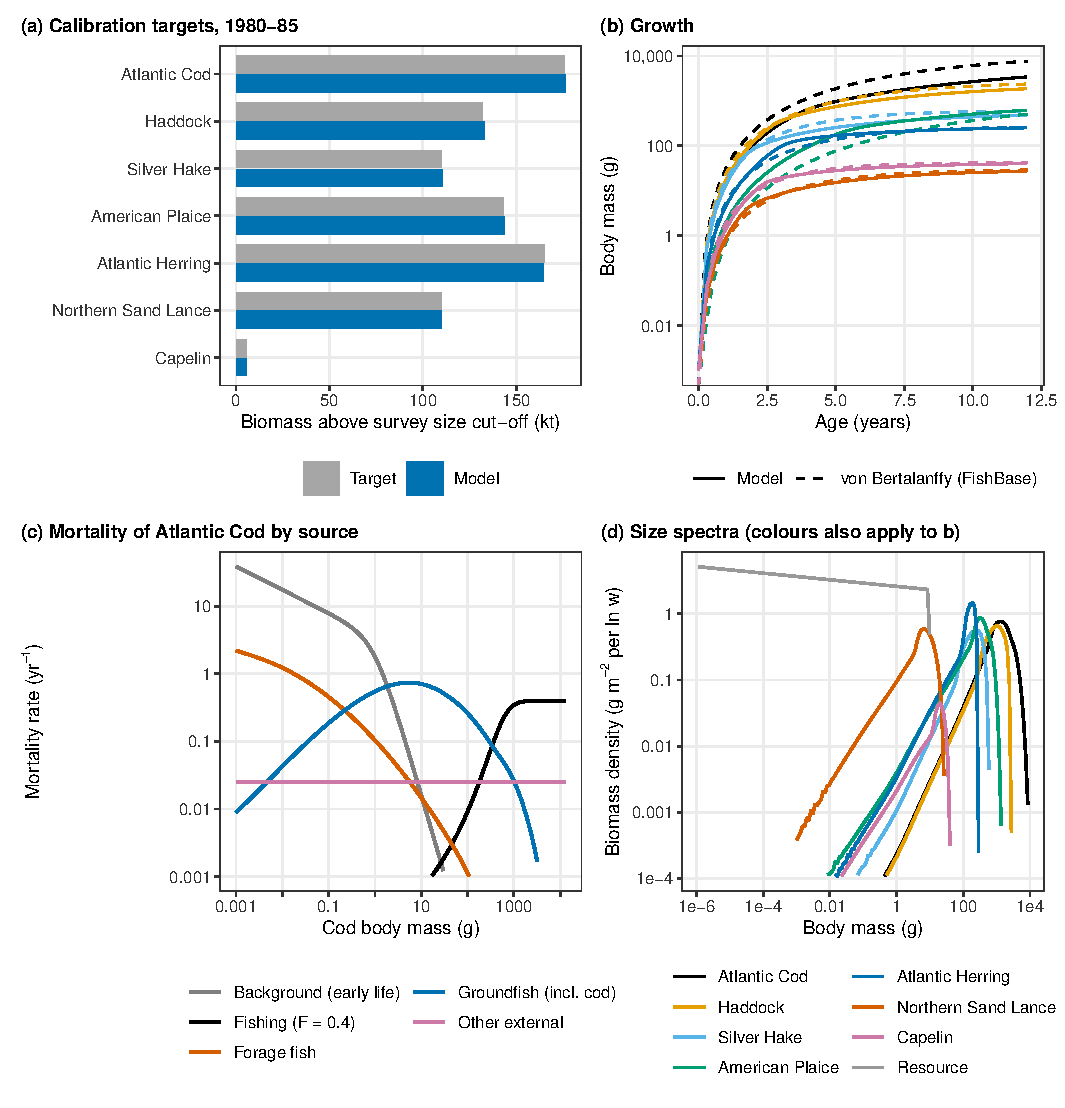
\includegraphics[width=\textwidth]{figures/fig1_baseline.pdf}
\caption{The calibrated 1980--85 steady state of the main model (v3, $s=20$). (a) Biomass above the survey size cut-off, model and calibration target (kt). (b) Modelled growth (solid) and von Bertalanffy curves from FishBase parameters (dashed); colours as in (d). (c) Mortality rate of cod by source and body mass: background early-life mortality (eq.~\ref{eq:bg}), predation by forage fish (including the vulnerability factor $s$), predation by groundfish, fishing at $F=0.40$ and other external mortality. (d) Biomass size spectra of the seven species and the plankton--benthos resource.}
\label{fig:baseline}
\end{figure}

\begin{figure}[p]
\centering
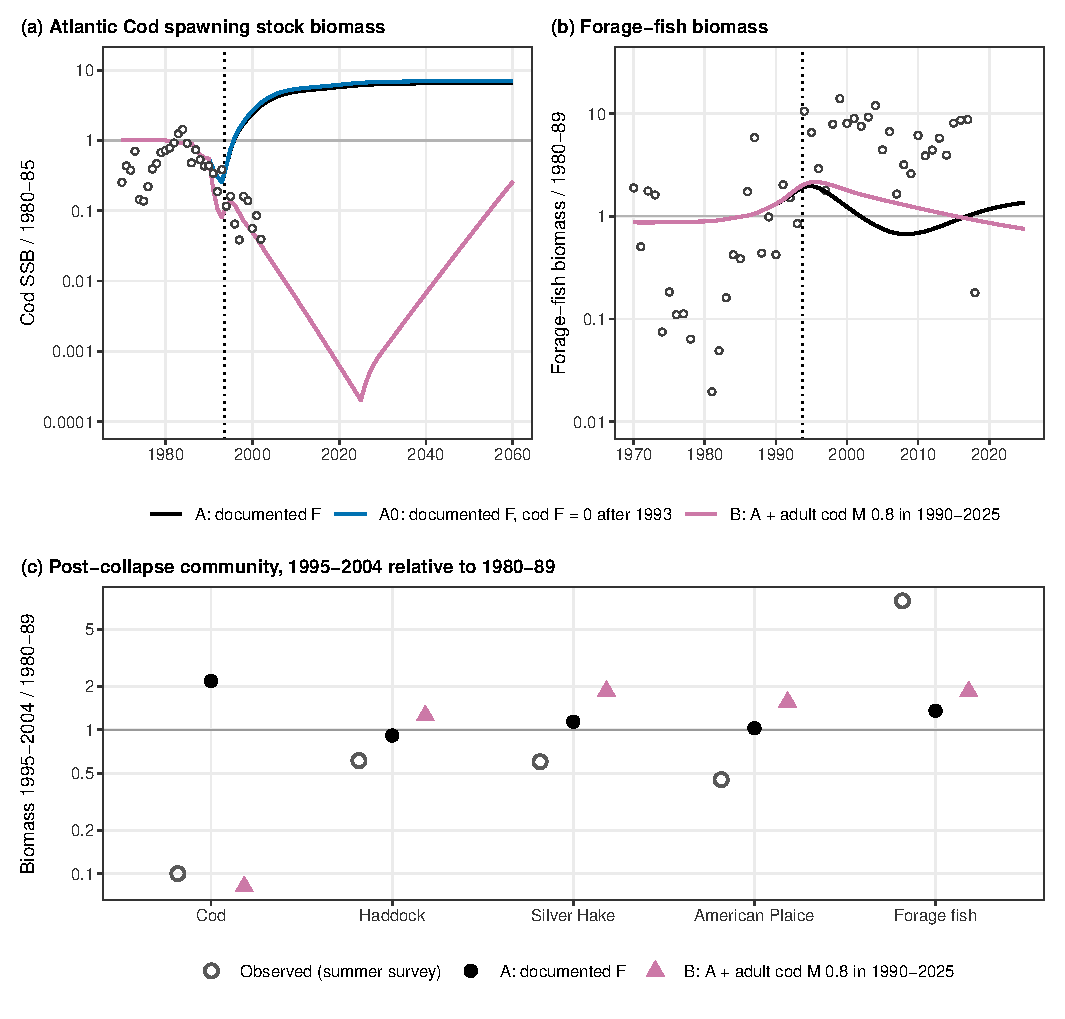
\includegraphics[width=\textwidth]{figures/fig2_hindcast.pdf}
\caption{Hindcasts with the documented fishing history (run~A; A0 with cod $F=0$ after 1993) and with adult cod natural mortality raised to 0.8~\yr{} in 1990--2025 (run~B, labelled alternative). (a) Cod spawning stock biomass relative to the model's 1980--85 baseline; open circles, survey-based SSB relative to its 1980--85 mean \autocite{fanning2003assessment}; dotted line, closure of the directed fishery (September 1993). After 2025 runs A and B continue at moratorium effort with baseline parameters. (b) Forage-fish biomass (herring, sand lance and Capelin) relative to its 1980--89 mean; open circles, summer survey, not catchability-adjusted \autocite{adekoya2026code}. (c) Ratio of mean biomass in 1995--2004 to 1980--89, observed (survey) and modelled (total biomass), logarithmic scale.}
\label{fig:hindcast}
\end{figure}

\begin{figure}[p]
\centering
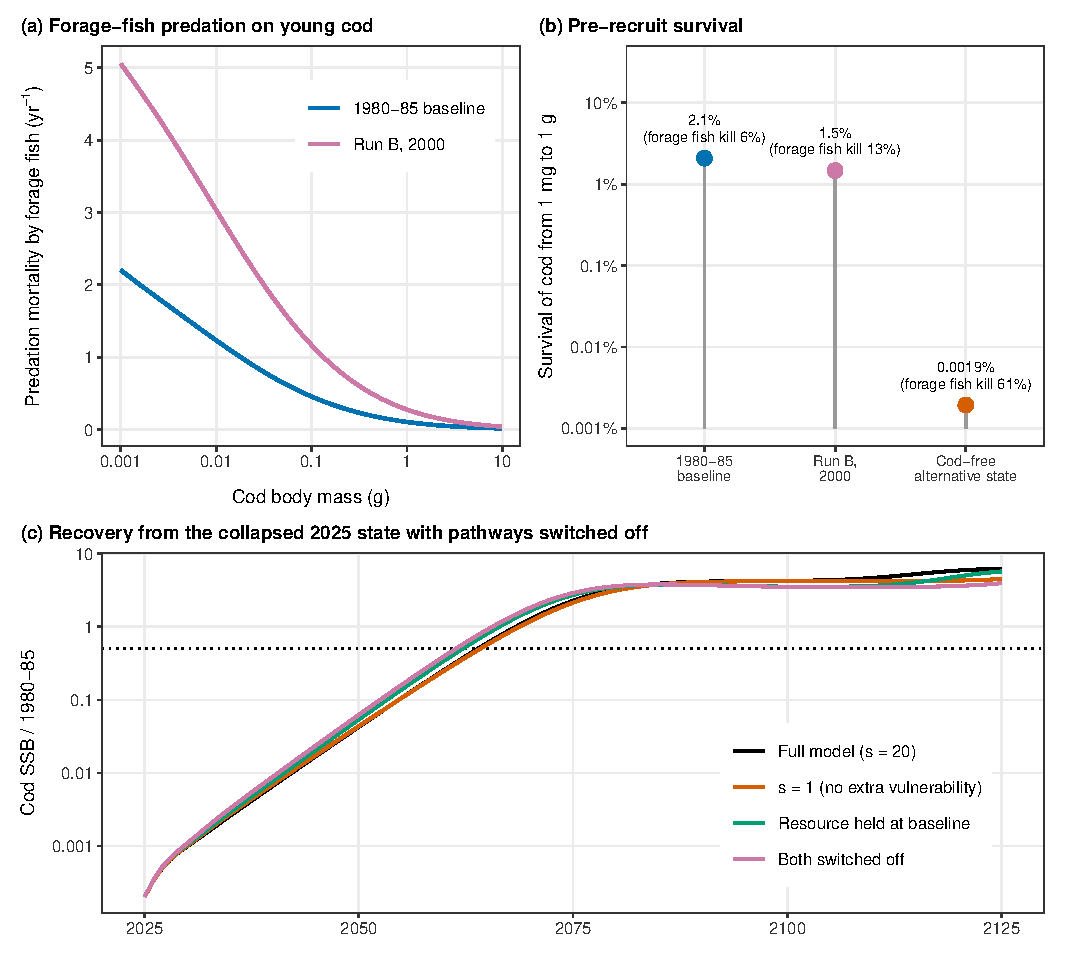
\includegraphics[width=\textwidth]{figures/fig3_pathways.pdf}
\caption{How strongly forage fish act on young cod. (a) Predation mortality of cod by forage fish as a function of cod body mass at the 1980--85 baseline and in the 2000 state of run~B (adult cod mortality 0.8~\yr{}). (b) Survival of a cod cohort from 1~mg to 1~g (eq.~\ref{eq:budget}) and the percentage of the cohort killed by forage fish, at baseline, in run~B in 2000 and in the model's cod-free alternative stable state (logarithmic scale). (c) Cod spawning stock biomass from the modelled collapsed 2025 state (run~B in 2025, baseline parameters, moratorium effort) in the full model and in diagnostic runs with $s=1$, with the resource held at its baseline abundance, or both; dotted line, 50\% of baseline.}
\label{fig:pathways}
\end{figure}

\begin{figure}[p]
\centering
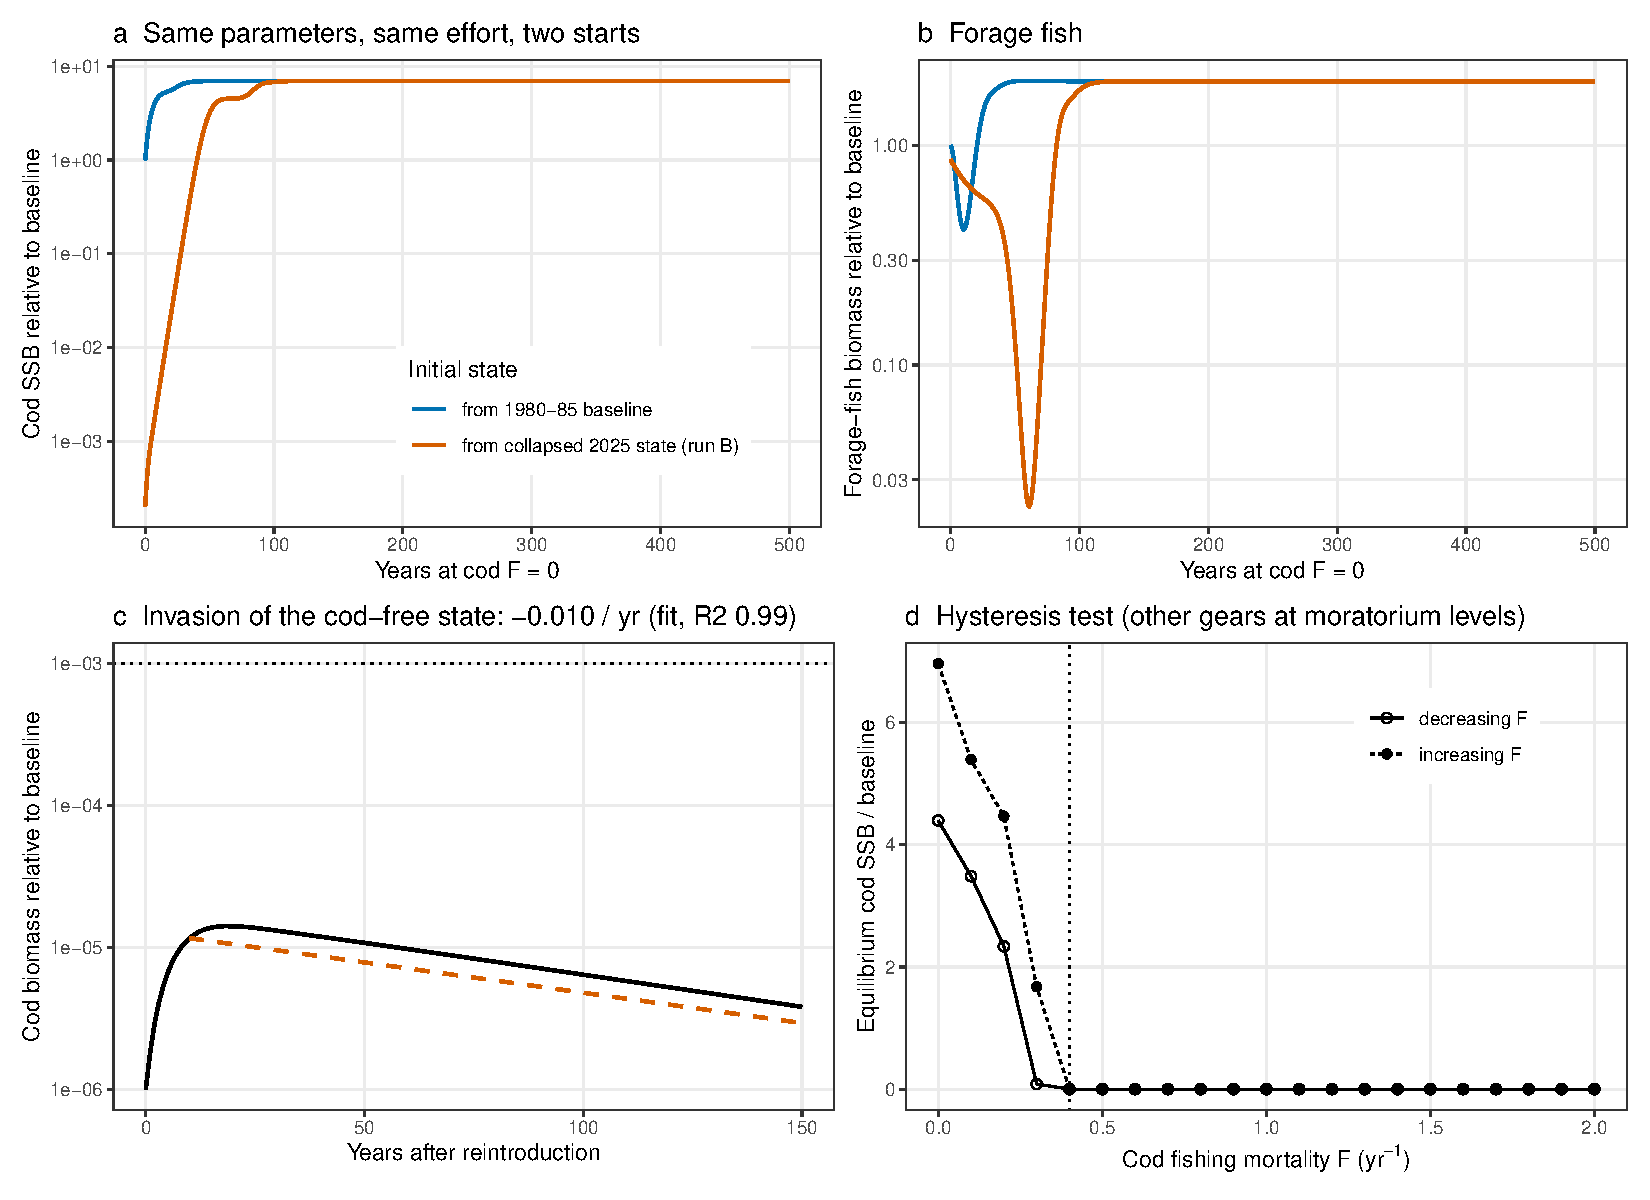
\includegraphics[width=\textwidth]{../figures/fig3_bistability.pdf}
\caption{Tests for alternative stable states at baseline parameters, cod $F=0$ and the other gears at moratorium levels. (a) Cod spawning stock biomass over 500 years from the 1980--85 baseline and from the modelled collapsed 2025 state (run~B). (b) Forage-fish biomass in the same runs. (c) Cod reintroduced at $10^{-6}$ of its baseline abundance into the equilibrium community without cod: biomass relative to baseline (solid) and the fitted per-capita growth rate over years 10--150 (dashed; slope $-0.0099$~\yr{}, $R^{2}=0.99$); dotted line, $10^{-3}$ of baseline. (d) Equilibrium cod SSB relative to baseline against cod $F$ for increasing (filled) and decreasing (open) $F$; in the decreasing sweep cod was reset to $10^{-3}$ of its baseline biomass whenever it fell below it; dotted line, baseline cod $F$ (0.40).}
\label{fig:bistability}
\end{figure}

\begin{figure}[p]
\centering
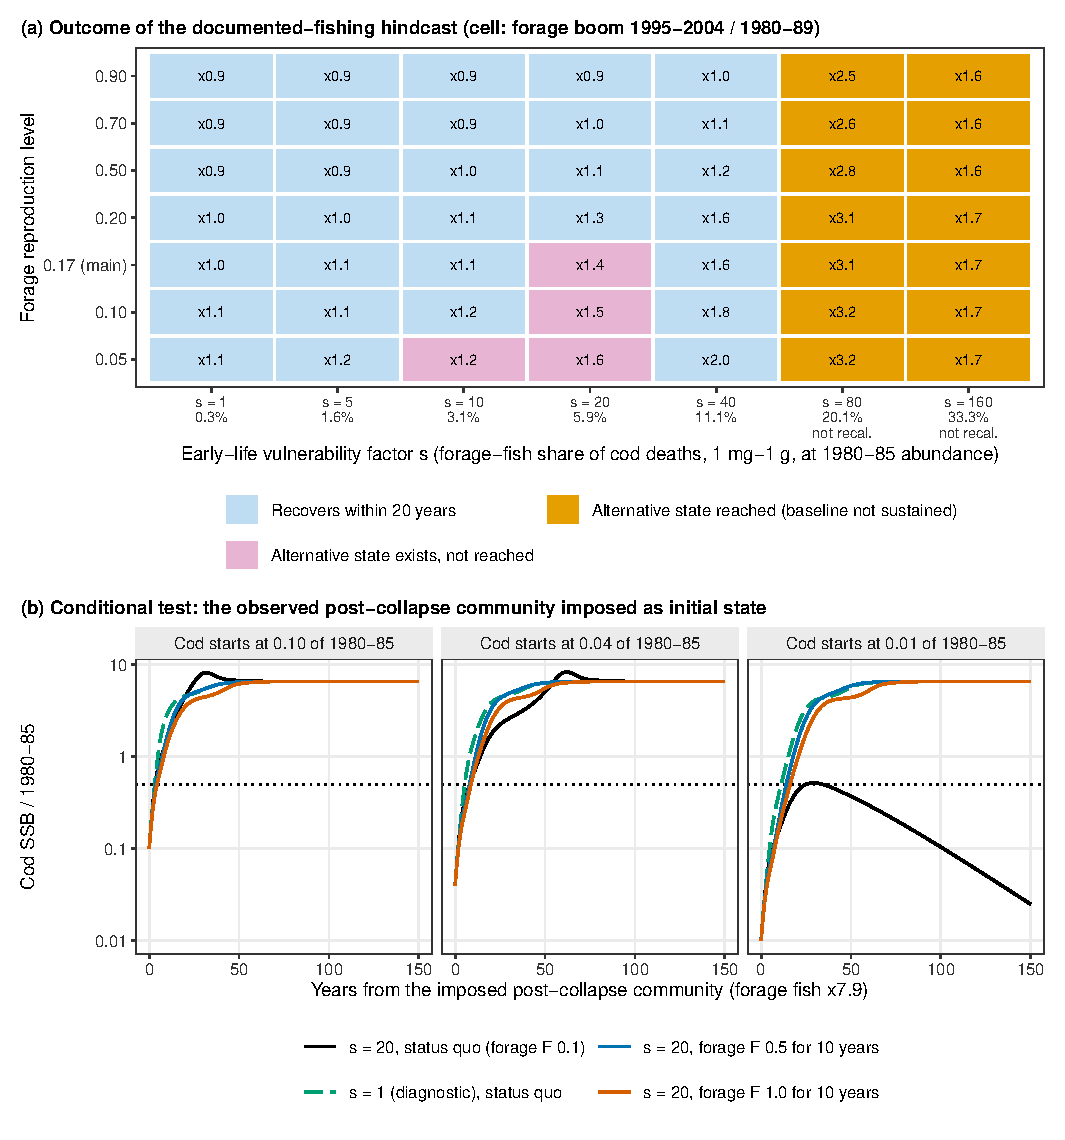
\includegraphics[width=\textwidth]{figures/fig5_what_it_would_take.pdf}
\caption{What it would take. (a) Outcome of the documented-fishing hindcast and of the invasion test for each combination of early-life vulnerability factor $s$ (with the share of cod deaths between 1~mg and 1~g caused by forage fish at 1980--85 abundance) and forage reproduction level; cell text, forage-fish biomass in 1995--2004 relative to 1980--89 (observed 7.87). Every recalibrated cell recovered to 50\% of baseline cod SSB within two years of 1993. $s=80$ and 160 could not be recalibrated; at those values the 1980s cod cannot persist at its 1980s fishing mortality. (b) Conditional test: the observed post-collapse community (forage fish 7.87 times, other groundfish 0.45--0.61 times their baseline) imposed as initial state, with cod at 0.10, 0.04 or 0.01 of its 1980--85 SSB; moratorium effort; $s=20$ with forage-fish $F$ at the status quo (0.1) or raised to 0.5 or 1.0 for 10 years, and $s=1$ as a diagnostic. Dotted line, 50\% of baseline SSB.}
\label{fig:wouldtake}
\end{figure}

\begin{figure}[p]
\centering
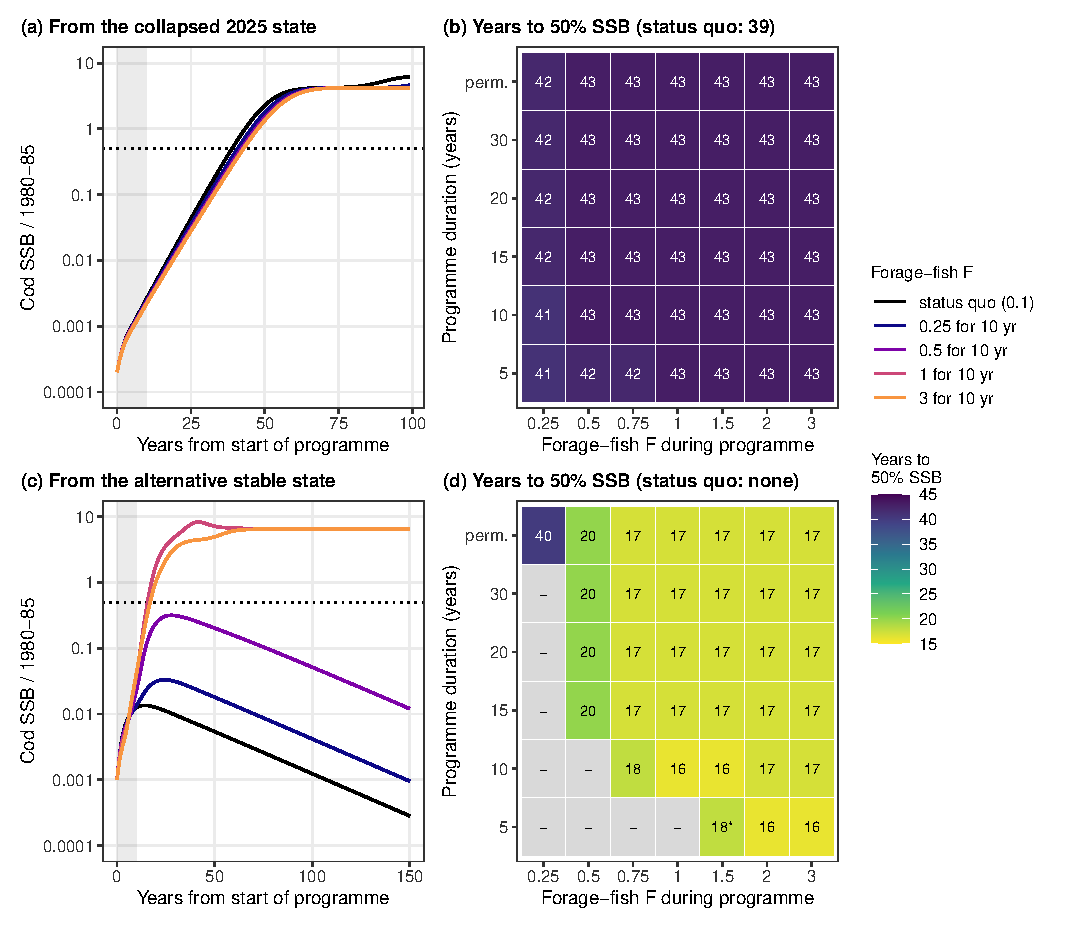
\includegraphics[width=\textwidth]{figures/fig6_forage_fishing.pdf}
\caption{Forage fishing as a recovery measure. (a, b) From the modelled collapsed 2025 state (run~B in 2025, adult mortality back at baseline). (c, d) From the model's alternative stable state, with cod and the other groundfish reintroduced at $10^{-3}$ of their baseline biomass. (a, c) Cod spawning stock biomass for the status quo (forage-fish $F$ 0.1) and for 10-year programmes (shaded) at forage-fish $F$ of 0.25--3; dotted line, 50\% of baseline. (b, d) Years from the start of the programme to 50\% of baseline cod SSB by forage-fish $F$ and programme duration; $-$, not reached within the run (100 or 150 years); $^{*}$, reached but not persistent. Cod $F$ is 0.02 and the other gears are at moratorium levels throughout.}
\label{fig:forage}
\end{figure}

\begin{figure}[p]
\centering
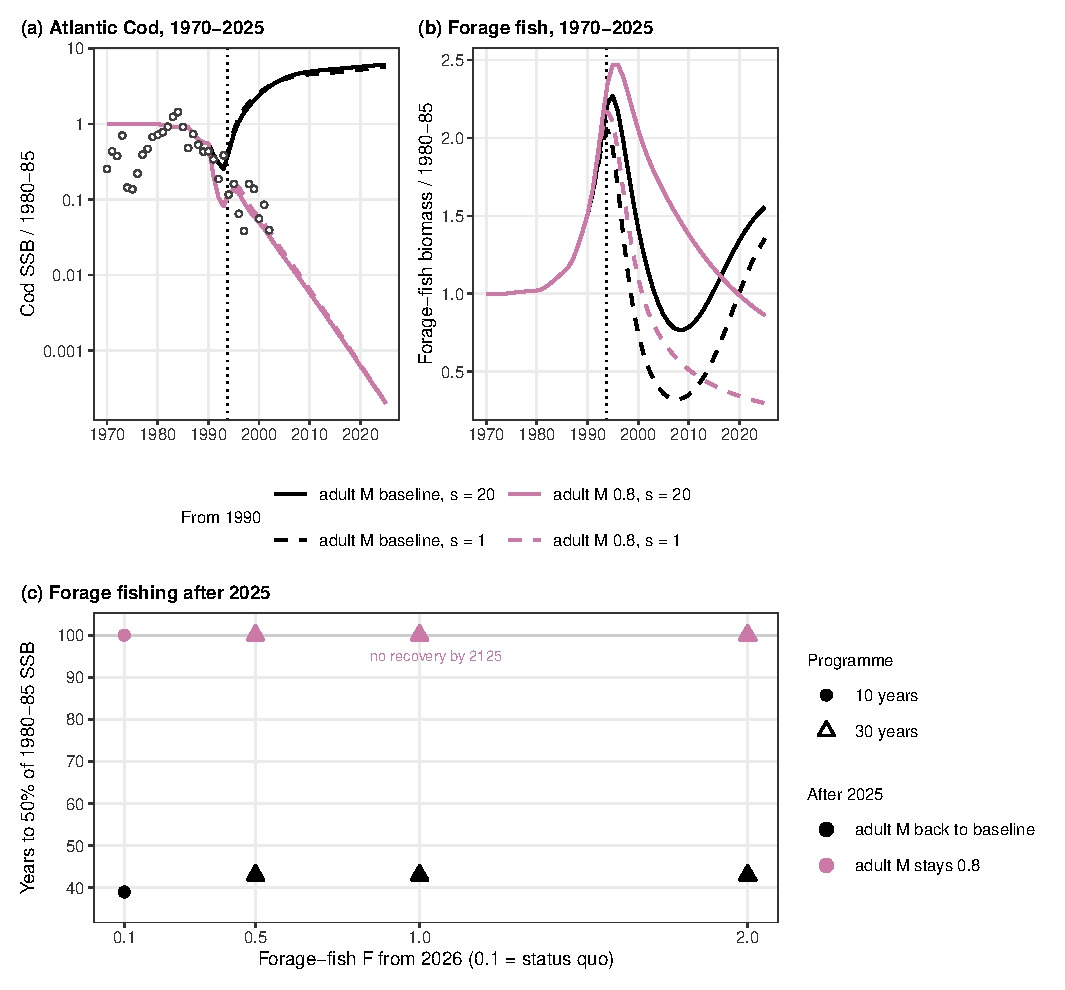
\includegraphics[width=\textwidth]{figures/fig7_adult_mortality.pdf}
\caption{Elevated adult natural mortality as the alternative explanation. (a, b) $2\times2$ factorial hindcast with the documented fishing history: adult cod (${\geq}35$~cm) natural mortality at baseline or 0.8~\yr{} from 1990, crossed with the forage mechanism ($s=20$) or the diagnostic $s=1$ from 1990. (a) Cod spawning stock biomass relative to 1980--85, with survey-based SSB \autocite[open circles;][]{fanning2003assessment}. (b) Forage-fish biomass relative to baseline. (c) Years from 2026 to 50\% of baseline cod SSB under forage-fishing programmes of 10 or 30 years started from the 2025 state of run~B, with adult mortality kept at 0.8 or returned to baseline in 2026; forage-fish $F$ 0.1 is the status quo. With adult mortality kept at 0.8, cod did not recover by 2125 in any programme.}
\label{fig:adultM}
\end{figure}


\end{document}
